% ============================================================================
%  APEX — RASTI manuscript (LaTeX, MNRAS class)
%  Generated from MANUSCRIPT.md, 2026-07-05.
%
%  HOW TO USE ON OVERLEAF (fastest path to a typeset PDF):
%   1. overleaf.com -> New Project -> Templates -> search "MNRAS" -> create.
%      (This gives you mnras.cls + mnras.bst so it compiles immediately.)
%      RASTI uses the same OUP/MNRAS layout; swap in RASTI's official class
%      later for final submission.
%   2. Replace the template's main .tex with THIS file (MANUSCRIPT.tex).
%   3. Upload references.bib (already prepared) into the project.
%   4. Upload the figures/ folder (includes fig_completeness_realvssynth.png and
%      fig_qc_depth.png alongside fig2_error_model.png ... fig9_crowded_field.png).
%   5. Menu -> Compiler: pdfLaTeX. Click Recompile.
%
%  Local build (if you have a TeX distribution + mnras.cls):
%   pdflatex MANUSCRIPT ; bibtex MANUSCRIPT ; pdflatex MANUSCRIPT ; pdflatex MANUSCRIPT
%
%  STATUS: full English draft. §4 is a reserved placeholder (awaits YZ Boo run).
%  TODO before submission: author list/affiliations, §4 content, back matter,
%  photutils version DOI, verify Paparó author list. See REFERENCES.md.
% ============================================================================
\documentclass[fleqn,usenatbib]{mnras}

\usepackage{graphicx}
\usepackage{amsmath}
\usepackage{amssymb}
\usepackage[T1]{fontenc}
\graphicspath{{figures/}}

\title[APEX: a validated graphical photometry pipeline]{APEX: a validated graphical pipeline for end-to-end aperture and PSF photometry from small telescopes}

% TODO: real author list + affiliations. Professor is a co-author ("we").
\author[Author et al.]{%
Author Name,$^{1}$\thanks{E-mail: author@example.edu}
and Advisor Name$^{1}$
\\
$^{1}$Affiliation, Institution, City, Country
}

\begin{document}
\label{firstpage}
\maketitle

\begin{abstract}
APEX (Automated Photometry EXtraction) is a desktop application that takes a non-specialist, through a graphical step-by-step workflow and without scripting, from raw CCD frames to a science product: a star-cluster colour--magnitude diagram or a multi-night variable-star light curve. It composes standard detection and photometry algorithms behind a graphical interface backed by a Qt-free, reproducible core, filling a gap between powerful command-line suites with a steep entry barrier and graphical tools scoped to single-field or transit photometry. Because the contribution is accessibility rather than a new algorithm, we validate the shared measurement chain in several independent layers, each checked against something the pipeline did not itself produce. Injected into real cluster frames, the detector's recovery collapses across seven frames of differing depth onto a single signal-to-noise threshold ($\mathrm{S/N}_{50}=4.05\pm0.18$), and on synthetic frames with known truth the reported uncertainties propagate correctly (pull standard deviation $1.014$). Two independently implemented engines agree with APEX to milli-magnitude precision, SEP on synthetic truth (MAD $0.006$ mag) and IRAF/DAOPHOT on a real 278-star frame (MAD $0.004$ mag). The pipeline's colour--magnitude diagram reproduces those of two independent instruments (main-sequence ridgeline agreement $19$ mmag); a faint-end anomaly is traced to a Gaia BP reference artifact rather than an APEX error; and re-reduction of two globular clusters shows no crowding-dependent bias between aperture and PSF photometry down to the resolution the data reach. We state explicitly what is not validated: automated isochrone-parameter recovery, photometry against strongly structured backgrounds, sub-resolution blending, and cross-instrument generality, as all data come from a single camera.
\end{abstract}

\begin{keywords}
techniques: photometric -- methods: data analysis -- software: development -- open clusters and associations: individual: NGC~457, NGC~6811 -- globular clusters: general -- stars: variables: $\delta$~Scuti
\end{keywords}

% ============================================================================
\section{Introduction}
\label{sec:intro}

Watching photometric software simply work leaves an impression. A student running exoplanet-transit photometry in a guided graphical tool such as HOPS \citep{tsiaras2019}, and obtaining a usable light curve in an afternoon, comes away expecting that turning a stack of CCD frames into calibrated stellar brightnesses is a solved, push-button task. For several common observing programmes on small telescopes, it is not yet that simple, and the gap between the expectation and the available tooling is the motivation for this work.

Two mature families of photometry software dominate practice. The first is the lineage of command-line reduction suites: DAOPHOT for crowded-field stellar photometry \citep{stetson1987} and SExtractor for source extraction \citep{bertin1996} remain standard, capable, and widely trusted. Their power comes at the cost of a steep entry barrier. Installation is nontrivial, much of the reference documentation predates current builds, and progress stalls at the many points where a parameter is ambiguous and the newcomer has no principled way to set it. The second family is the modern scientific-Python stack, where \texttt{photutils} \citep{photutils} on top of Astropy \citep{astropy2013, astropy2018, astropy2022} offers flexible, well-tested primitives. That flexibility presumes the user can write the script that orchestrates them. Between these sits a set of graphical tools that trade generality for guidance, but each is scoped to a particular problem: AstroImageJ \citep{collins2017} and HOPS \citep{tsiaras2019} are built around single-field differential and transit photometry, while variable-star packages such as Munipack/MuniWin \citep{hroch2014} and VStar \citep{benn2012} target time-series analysis and are, in the authors' experience, difficult to approach without prior familiarity.

The result is a missing path. No widely used graphical tool guides a non-specialist from raw frames all the way to a finished science product for two of the most common small-telescope programmes that the tools above do not jointly cover: a star-cluster colour--magnitude diagram (CMD) and a multi-night variable-star light curve. Each of these requires the same unglamorous measurement chain (detection, astrometric solution, a master source catalogue, and forced photometry at fixed positions) before any science-specific step, and it is precisely that shared chain, together with a guided route through it, that the newcomer lacks.

APEX (Automated Photometry EXtraction) is built to fill this gap. It is a desktop application that carries a user, through a graphical step-by-step workflow, from image selection to either a cluster CMD or a variable-star light curve. Two operational modes share a common measurement chain and then branch: a CMD mode for cluster photometry and a light-curve (LC) mode for multi-night differential photometry and period analysis. The shared chain performs source detection, WCS plate solving, master-catalogue construction, and forced aperture and PSF photometry, using standard algorithms drawn from the lineage above rather than new ones. A deliberate architectural choice separates the graphical layer from a Qt-free computational core, so that every reduction step can also be run headlessly and reproducibly; the same core that backs the interface is exercised, unchanged, in the validation experiments of this paper.

It is worth stating plainly who this is for, and why a new tool is worth any risk at all. Anyone already fluent in DAOPHOT or able to write \texttt{photutils} scripts should keep using them; APEX does not claim to do those jobs better. The user we build for has not reached that point but wants to work with their own data the way a scientist does: an undergraduate or beginning graduate student, an observer with a small telescope, a serious amateur moving from imaging to measurement. For that user the obstacle is not a missing algorithm but a missing path --- which parameter to set, what a defensible value looks like, and whether the number that finally comes out can be trusted. A graphical workflow answers the first two by construction, and Section~\ref{sec:chain} describes the chain as a sequence of such decisions rather than of buttons. The third it cannot answer merely by being convenient, and an easy tool that is quietly wrong is worse than a difficult one that is right --- that is the real risk of this category of software. It is why roughly half of this paper measures the tool instead of describing it: Sections~\ref{sec:validation} and~\ref{sec:science} are our answer to \emph{why accept the risk}, in that the shared chain agrees with an independent engine to milli-magnitudes, reports errors that match its own scatter, predicts each frame's detection depth before measuring it, and recovers a published pulsation period from raw frames through the graphical workflow alone.

Because APEX composes established algorithms rather than introducing new ones, its contribution is not algorithmic novelty. It is accessibility paired with demonstrated trustworthiness, in the spirit of automated-pipeline papers such as AutoPhOT \citep{brennan2022}. Concretely, this paper contributes: (i) a description of an integrated, graphical, end-to-end photometry pipeline that reaches cluster-CMD and multi-night light-curve science products without scripting; and (ii) a multi-layer, reproducible validation of its shared measurement chain, in which every accuracy claim is checked against something the pipeline did not itself produce, an independent measurement engine, an independent reference catalogue, or an injected known truth. We regard the second contribution as inseparable from the first: modern AI-assisted development has lowered the barrier to \emph{building} scientific software as much as graphical tools lower the barrier to \emph{using} it, and that shift makes independent, reproducible validation not an optional flourish but the precondition for trusting such a tool at all.

The remainder of this paper is organised as follows. Section~\ref{sec:design} describes APEX's design and the shared measurement chain. Section~\ref{sec:validation}, the core of the paper, presents the validation suite. Section~\ref{sec:science} demonstrates the pipeline end to end on a variable-star science case. Section~\ref{sec:discussion} discusses what the validation does and does not establish, and Section~\ref{sec:conclusion} concludes.

% ============================================================================
\section{Design and implementation}
\label{sec:design}

\subsection{Architecture}

APEX is organised around a deliberate split between a graphical presentation layer and a Qt-free computational core. The graphical layer, built on PyQt5, presents the workflow as an ordered sequence of step windows and owns every interactive element: file selection, crop definition, the sky-preview image viewer, and the mode-specific analysis steps. The numerically substantial steps, source detection, astrometric solution, and forced photometry, live in a separate core (\texttt{apex.analysis}, orchestrated by \texttt{apex.pipeline}) that imports no Qt and can be driven headlessly. This is not an aspirational refactor. The same core functions that back the interface are called directly, unchanged, by the benchmark and validation harness used throughout Section~\ref{sec:validation}, so that what is validated is exactly what the interface runs. A headless pipeline runner plans the step sequence, checks prerequisites, executes steps idempotently, and writes a JSON run manifest; that runner is what makes the reproductions of Section~\ref{sec:validation} possible.

Two operational modes share the first seven steps and then branch. CMD mode continues to cluster-specific analysis (PSF photometry, calibration, the colour--magnitude diagram, and isochrone modelling); LC mode continues to differential light-curve construction, multi-night detrending, and period analysis. Because the shared chain is what this paper validates, we describe it in detail and the mode branches only briefly.

\subsection{The shared measurement chain (Steps 1--7)}
\label{sec:chain}

Steps 1--3 prepare the data. FITS files are selected and their headers scanned to resolve the target and instrument, a common crop region is defined on a reference frame and applied to the stack, and a sky-preview step provides interactive inspection together with an automatic frame quality-control evaluation (validated in Section~\ref{sec:qc}).

Source detection (Step 4) uses image segmentation from \texttt{photutils} \citep{photutils, astropy2022}: sources are found with \texttt{detect\_sources} above a configurable threshold, separated with \texttt{deblend\_sources}, and optionally refined with \texttt{DAOStarFinder}, with three presets (normal, crowded, faint) selecting the detection parameters. The detector is a single implementation shared by the interface and the headless core.

Astrometric calibration (Step 5) solves each frame's world-coordinate system with a local ASTAP solve \citep{astap}, falling back automatically to a local astrometry.net solve \citep{lang2010} when ASTAP is unavailable; coordinate transformations use \texttt{astropy.wcs} \citep{astropy2013}. Step 6 merges the per-frame detections into a single master source catalogue, which fixes the positions at which every frame is subsequently measured.

Forced aperture photometry (Step 7) measures every master source in every frame at its catalogue position. Fluxes are integrated in a circular aperture with fractional-pixel weighting and the sky is estimated in a concentric annulus, using \texttt{photutils} apertures \citep{photutils}. The default aperture radius scales with the frame's measured FWHM, $r_{\rm ap} = \max(4\,{\rm px},\, 0.8\,{\rm FWHM})$, and the sky annulus spans roughly 4--6~FWHM; all radii are configurable, and Section~\ref{sec:sweep} examines the aperture choice empirically. Uncertainties follow the full CCD equation, combining source and background Poisson noise, background-estimation error, and read noise; the honesty of these reported uncertainties is tested in Section~\ref{sec:errormodel}. Photometry is vectorised over the sources within a frame and parallelised over frames, with a worker count set by the host machine (75 per cent of cores, bounded above), so that a night of several hundred 16-megapixel frames reduces in a single pass.

Instrumental magnitudes are defined as a count rate, $m_{\rm inst} = 25 - 2.5\log_{10}(F_e / t_{\rm exp})$, which is exposure-time invariant. Absolute calibration (in CMD mode, Step 10) proceeds from these instrumental magnitudes through a per-frame zeropoint and an optional colour term to an absolute scale anchored on Gaia DR3 \citep{gaia_dr3_2023} reference stars, with astrometric and photometric quality cuts (the RUWE index and the corrected BP/RP flux-excess factor $C^*$; \citealt{riello2021}). Frame-to-frame offsets and atmospheric extinction are separated by projecting the frame-offset basis to remove the component degenerate with airmass.

\subsection{Mode-specific analysis}

After Step 7 the two modes diverge. In CMD mode, an optional PSF-photometry step (Step 8) builds an empirical point-spread function from bright, isolated stars in each frame using the \texttt{photutils} EPSF machinery and remeasures sources by PSF fitting; when it is skipped, downstream steps fall back to the forced-aperture results. Calibration (Step 10), the colour--magnitude diagram (Step 11), and isochrone modelling (Step 12) follow. In LC mode, the user selects target and comparison stars (Step 8), builds differential light curves (Step 9), detrends and merges nights (Step 10, using the SYSREM algorithm; \citealt{tamuz2005}), and searches for periods (Step 11, by Lomb--Scargle and phase-dispersion minimization; \citealt{stellingwerf1978}). This paper validates the shared chain and, in Section~\ref{sec:cmd}, the CMD product; isochrone-parameter recovery and LC-mode period recovery are treated separately (Sections~\ref{sec:science} and~\ref{sec:outofscope}), and we are careful not to present the mode-specific steps as validated beyond what Sections~\ref{sec:validation} and~\ref{sec:science} actually establish.

\subsection{Reproducibility and configuration}

All runtime parameters are read from a single TOML file, keeping instrument, detection, solving, and photometry settings in one auditable place. Pipeline state, which steps have run and with what data, is persisted as JSON, and every step's outputs are written to canonical paths derived from a small set of path helpers rather than assembled ad hoc, so that a result tree is self-describing and re-enterable. Cached intermediate products (header scans, detections, photometry) carry a signature and a schema version and are invalidated when a governing parameter changes, which prevents stale results from surviving a configuration change. Together these make a reduction reproducible from the parameter file and the input frames alone, the property on which Section~\ref{sec:validation} depends.

% ============================================================================
\section{Validation}
\label{sec:validation}

\subsection{Approach and data}

Every result in this section checks APEX against something it did not itself produce: an injected known truth, an independently implemented measurement engine, or an independent reference catalogue. No script fits a free parameter to the data it then judges; zeropoints and colour terms are always solved on an independent bright-star subset before residuals are examined at the faint end. We include the one investigation that turned up a genuine discrepancy (Section~\ref{sec:refcheck}) precisely because a validation exercise that reports only confirmations is not a validation.

Two kinds of experiment appear below. The detection-completeness test (Section~\ref{sec:completeness}) injects artificial stars into seven real frames of the clusters M67, NGC~6811 and M13, keeping a synthetic frame only as a numerical-verification control. The other self-contained synthetic experiments (Sections~\ref{sec:errormodel}--\ref{sec:sepcheck} and~\ref{sec:qc}) render a population of stars over a Poisson-plus-Gaussian noise background with a realistic FITS header, entirely in \texttt{numpy} and \texttt{astropy} \citep{astropy2013, astropy2022}, from APEX's own synthetic-frame generator with a fixed seed and no external data. Artificial-star injection uses an empirical PSF extracted from the frame itself and reruns APEX's production, Qt-free detector, not a toy re-implementation. The real-data cross-checks (Sections~\ref{sec:irafcheck}, \ref{sec:refcheck}--\ref{sec:crowding}) use previously reduced APEX result trees for the open clusters NGC~457 and NGC~6811 and the globular clusters M5 and M13, each re-run through the current headless code immediately before its figure was produced, so all real-data results reflect the current codebase rather than an archived one. One caveat, verified from FITS headers rather than assumed, governs the whole section: every real dataset used here was taken with a single camera (Section~\ref{sec:generality}).

\subsection{Detection completeness}
\label{sec:completeness}

\begin{figure*}
  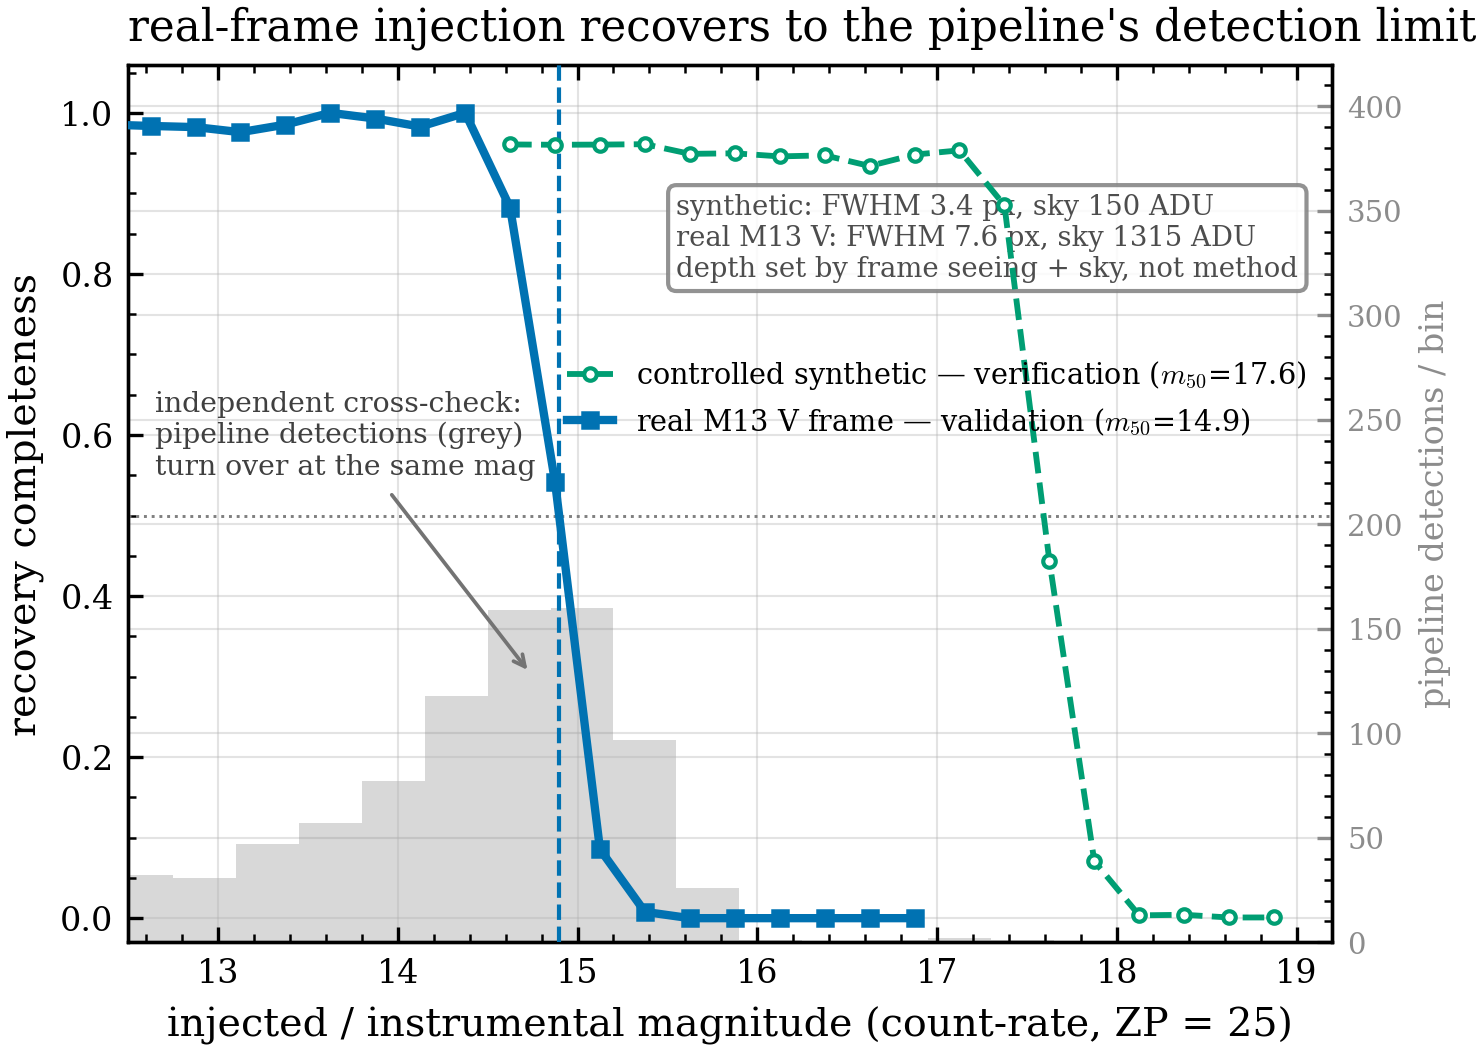
\includegraphics[width=\textwidth]{fig_completeness_realvssynth.png}
  \caption{Detection completeness by injection into real frames. \emph{(a)} Recovery fraction versus injected magnitude (count-rate system, ZP$\,=25$; Wilson-95 per cent binomial points, no curve fitted in magnitude space) for three representative single exposures spanning the observed conditions --- dark/sharp (M67~$i$), bright/sharp (NGC~6811~$R$), bright/soft (M13~$V$). The 50 per cent depths $m_{50}=17.65,\,15.64,\,14.90$ are read off the crossings and are a property of each frame's sky and seeing, not of the method; the synthetic verification frame (grey dashed) locates the machinery, not the depth. The strip shows real injected stars in the shallowest frame straddling its transition. \emph{(b)} Re-expressed by each source's expected peak-pixel signal-to-noise, all seven frames collapse onto one law: a pooled error-function fit gives $\mathrm{S/N}_{50}=4.0$, with independent per-frame read-offs $4.05\pm0.18$.}
  \label{fig:completeness}
\end{figure*}

Completeness sets the effective depth of any catalogue APEX builds. We run the artificial-star test of DAOPHOT's \textsc{addstar} \citep{stetson1987} in its modern real-frame form \citep[cf.][]{anbajagane2025, brennan2022}: 3000 stars are injected into each of seven real single exposures (three clusters, 60--480~s) spanning a factor 11 in background noise ($\sigma=5$--$58\,e^-$\,px$^{-1}$) and 1.7 in seeing (FWHM 5.2--9.0~px), each carrying the frame's own empirical PSF and source Poisson noise, and recovered through the production detector. Read off where the binned recovery crosses one half, the 50 per cent depths are $m_{50}=17.65$, $15.64$ and $14.90$ for the three frames of Fig.~\ref{fig:completeness}a: depth is a property of the frame --- its sky and seeing --- not of the method, and the count-rate system makes exposures of different length directly comparable. The controlled synthetic frame is kept only as a verification that the recovery machinery is numerically correct; its depth resembling the best real frame is a coincidence of a higher background offset by a sharper PSF, not a correspondence of conditions.

What the pipeline controls is not a magnitude but a signal-to-noise ratio. Re-expressing every injected star by its expected peak-pixel S/N --- the injected flux times the PSF peak fraction, divided by the frame's background noise --- collapses all seven frames, spanning 3.4 mag of depth, onto a single completeness law (Fig.~\ref{fig:completeness}b). An error-function detection-probability form \citep{masci2011, kashyap2010} fitted to the pooled sample gives $\mathrm{S/N}_{50}=4.0$, with independent per-frame read-offs $4.05\pm0.18$ (4 per cent frame-to-frame); this sits above the nominal $3.2\sigma$ per-pixel threshold because the detector requires a source to clear it over a minimum connected area. The measured completeness is predictive: applied to the master-catalogue stars on a frame it recovers the number the pipeline actually detected to within 6 per cent. Absolute depth is thus a property of the frame while the recovery S/N is invariant across conditions, and the magnitude-space curves are this one law shifted by each frame's $\sigma\cdot\mathrm{FWHM}^2$.

\subsection{Photometric error model}
\label{sec:errormodel}

\begin{figure}
  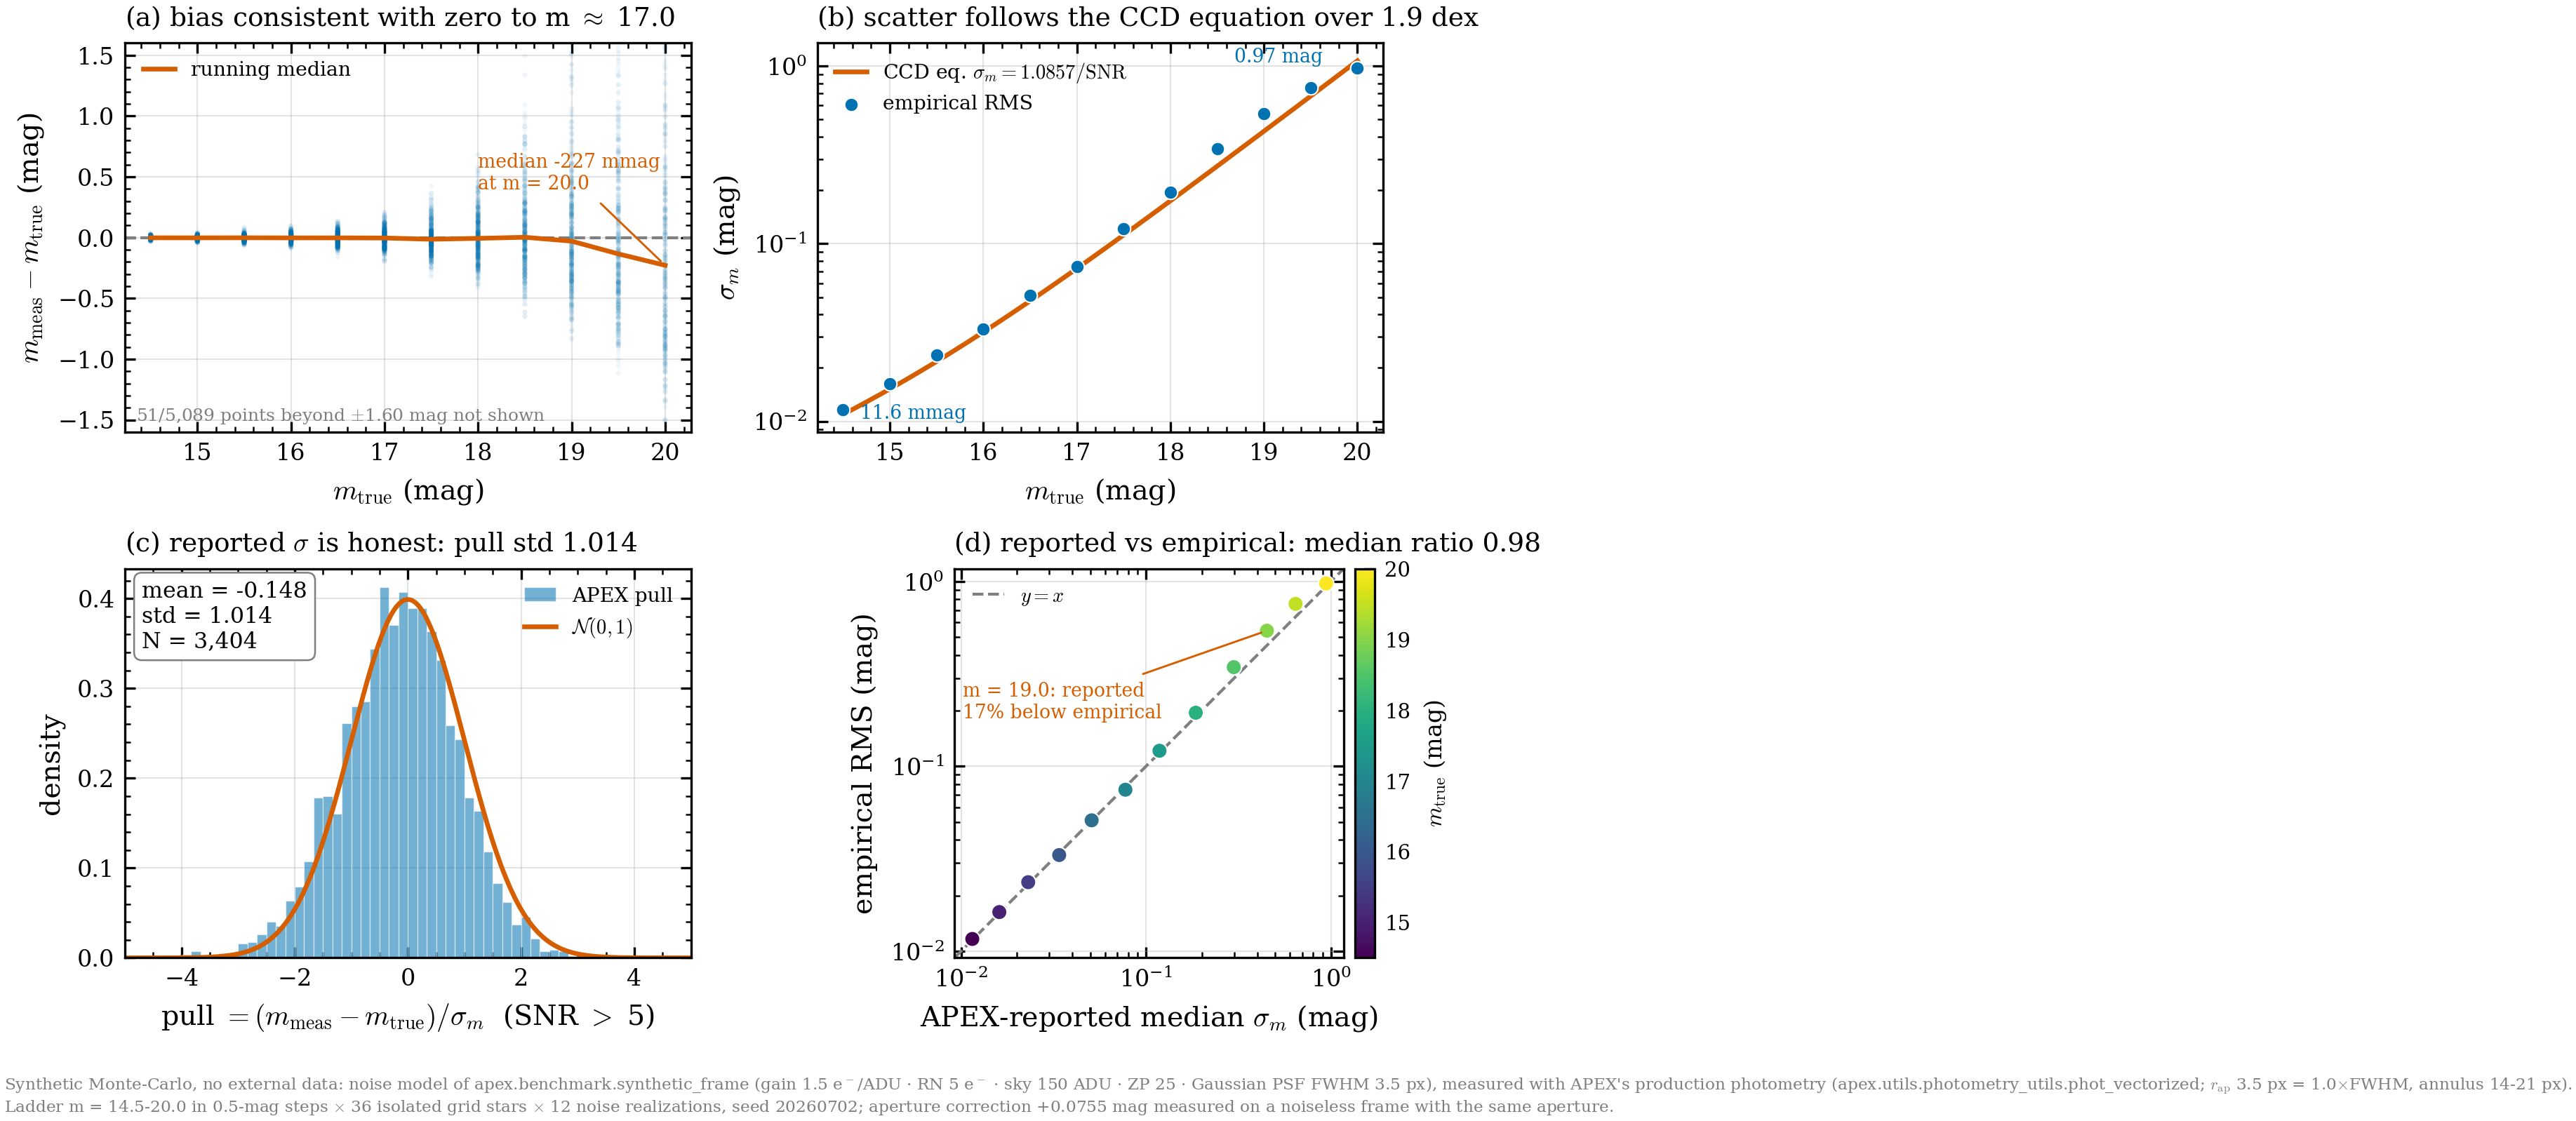
\includegraphics[width=\columnwidth]{fig2_error_model.png}
  \caption{Controlled Monte-Carlo validation of the reported uncertainties. The pull $(m_{\rm meas}-m_{\rm true})/\sigma_m$ for SNR$>5$ is a unit Gaussian (mean $-0.15$, standard deviation $1.014$, $N=3404$).}
  \label{fig:errormodel}
\end{figure}

On a well-separated grid injected across $m=14.5$--$20.0$ and re-measured, the uncertainties reported by the photometry match the recovered scatter (Fig.~\ref{fig:errormodel}). The bias is consistent with zero to $m\approx18.5$; the per-bin RMS follows the CCD relation $\sigma_m = 1.0857/{\rm SNR}$ across two decades; and the pull $(m_{\rm meas}-m_{\rm true})/\sigma_m$ for SNR~$>5$ is a unit Gaussian (mean $-0.15$, standard deviation $1.014$, $N=3404$). Reported and empirical uncertainties track along $y=x$ to a median ratio of $0.98$, with a mild $\sim$15 per cent under-estimate only at the faintest bins, attributable to the nonlinear magnitude transform near the detection floor. This experiment establishes that the pipeline \emph{propagates} its assumed noise model correctly; that the assumed model matches a real detector is a separate question, supported indirectly by the real-data cross-checks below (Sections~\ref{sec:irafcheck}, \ref{sec:crowding}), where the measured scatter between APEX and an independent engine is consistent with the reported uncertainties.

\subsection{Parameter and observing-condition sensitivity}
\label{sec:sweep}

\begin{figure}
  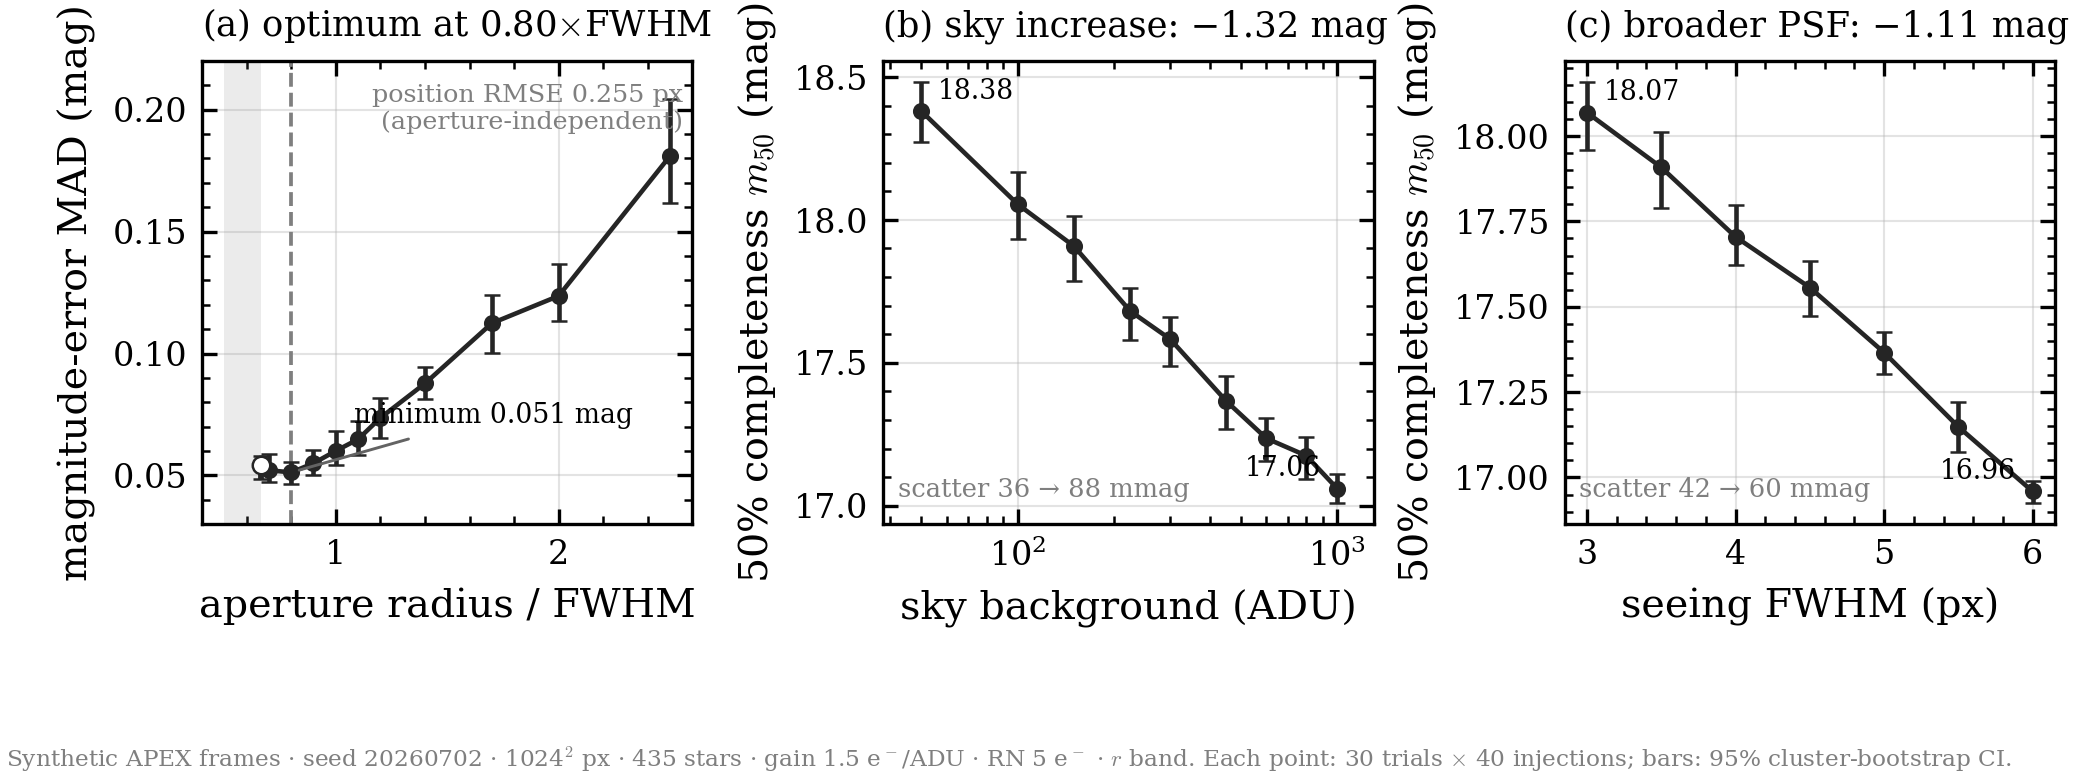
\includegraphics[width=\columnwidth]{fig3_parameter_sweep.png}
  \caption{Sweeps of aperture radius, sky background, and seeing. Scatter is minimized near $1.2\times$FWHM; depth shallows monotonically as sky brightens and seeing worsens.}
  \label{fig:sweep}
\end{figure}

Sweeping the pipeline and the observing conditions moves the metrics in the physically expected directions (Fig.~\ref{fig:sweep}). Photometric scatter as a function of aperture radius is minimized near $1.2\times$FWHM, while position RMSE is aperture-independent (set by detection, not aperture). The 50 per cent depth shallows monotonically as the sky brightens ($m_{50}$ from 18.48 to 17.11 mag over 50--1000 ADU) and as the seeing worsens (18.09 to 16.79 mag over FWHM 2.5--6.0 px). A companion sweep shows the detector is threshold-robust: $m_{50}$ is constant to $<0.01$ mag with zero spurious detections across detection thresholds of 2--6$\sigma$ on a clean field, so recovery is set by SNR, not by the threshold. The empirical aperture optimum near $1.2\times$FWHM sits close to the shipped default (Section~\ref{sec:chain}).

\subsection{Independent-engine cross-check on synthetic truth}
\label{sec:sepcheck}

\begin{figure}
  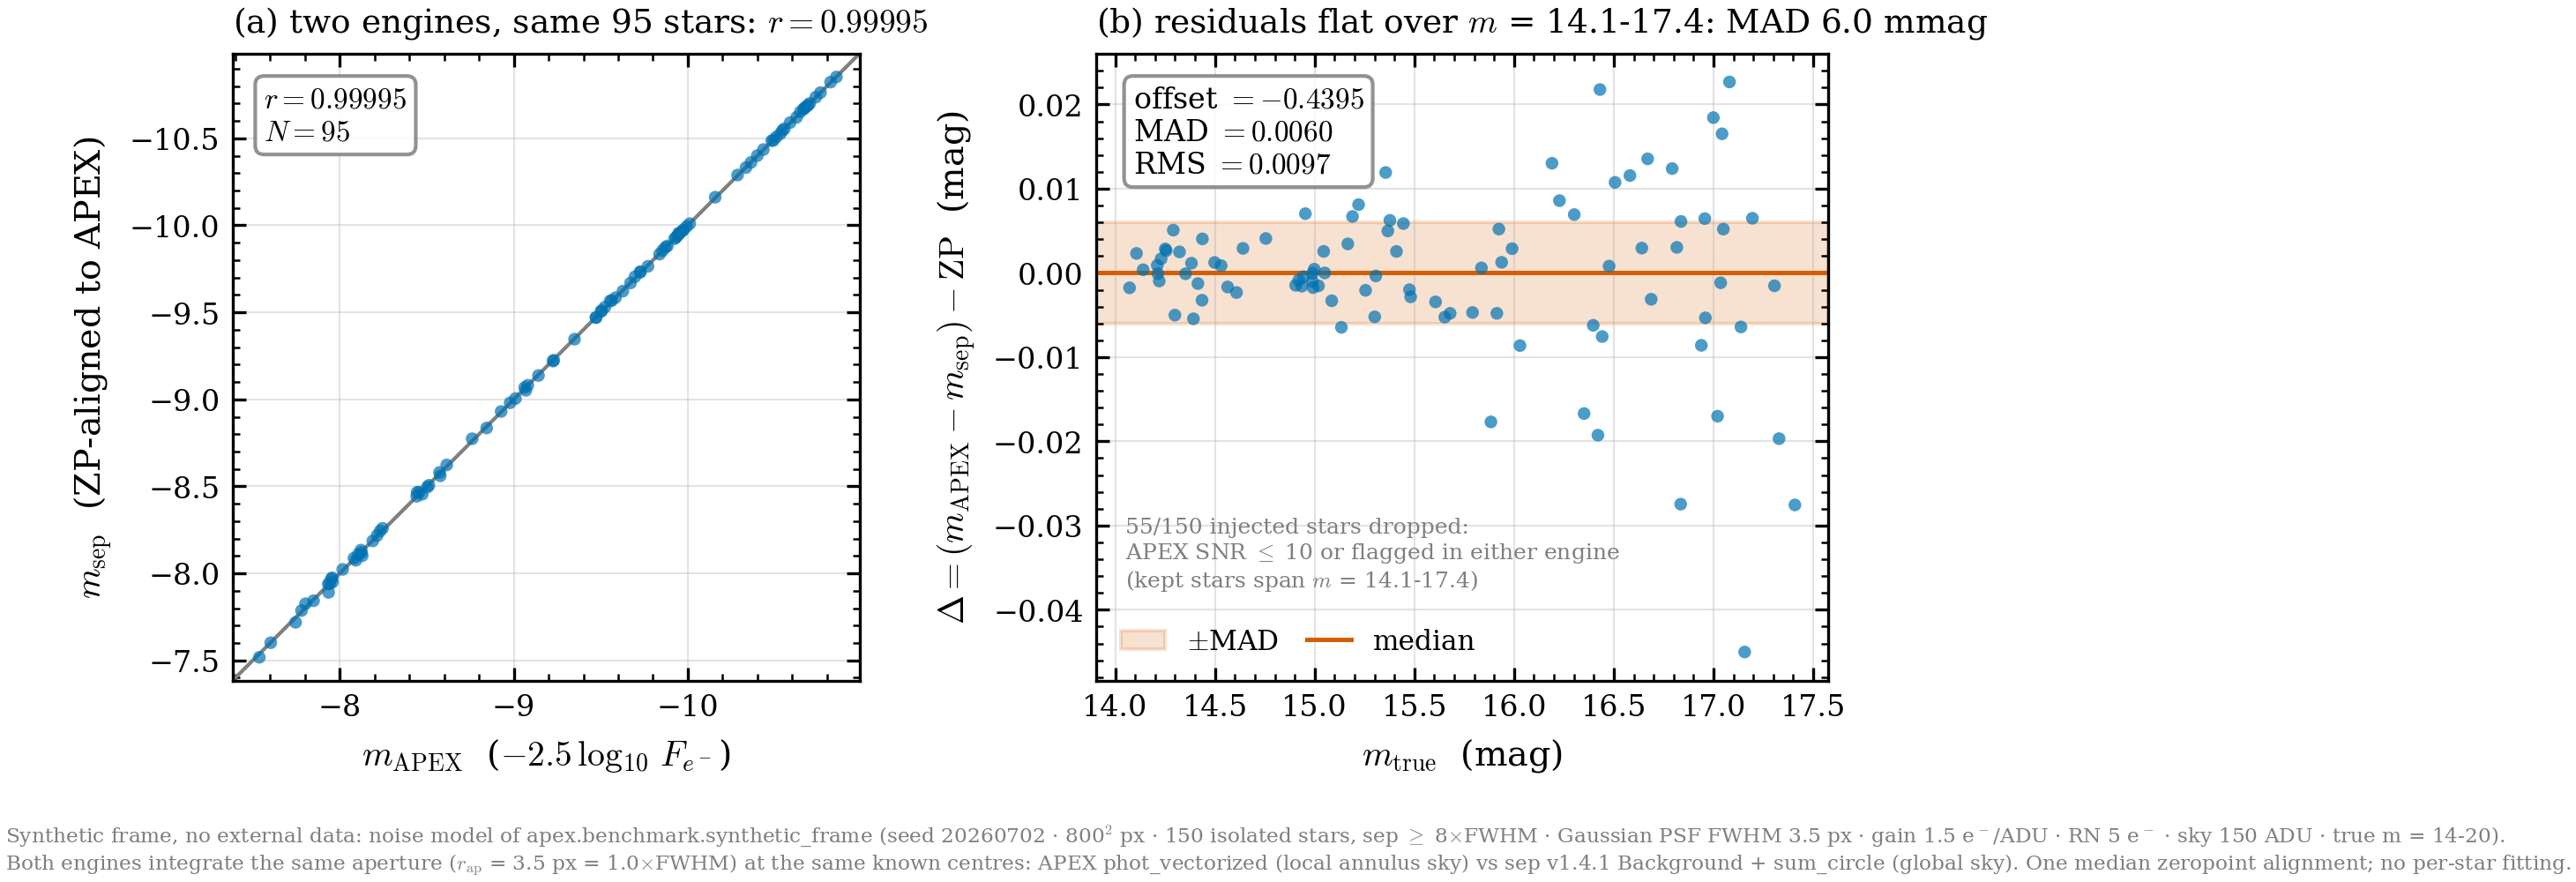
\includegraphics[width=\columnwidth]{fig4_crosscheck_sep.png}
  \caption{APEX versus the independent SEP engine on a synthetic frame with known truth: MAD $0.0060$ mag, $r=0.99995$ after a single zeropoint alignment.}
  \label{fig:sepcheck}
\end{figure}

Measuring the same 95 well-detected stars in one synthetic frame (known truth) independently with APEX and with Barbary's SEP library (a standalone SExtractor backend that shares no code with APEX; \citealt{bertin1996}) gives photometric-grade agreement after a single zeropoint alignment: MAD $0.0060$ mag, RMS $0.0097$ mag, Pearson $r=0.99995$, with 95 per cent of stars agreeing within 0.02 mag (Fig.~\ref{fig:sepcheck}). Two independently implemented engines therefore return the same fluxes on the same pixels.

\subsection{Independent-engine cross-check on real data}
\label{sec:irafcheck}

\begin{figure}
  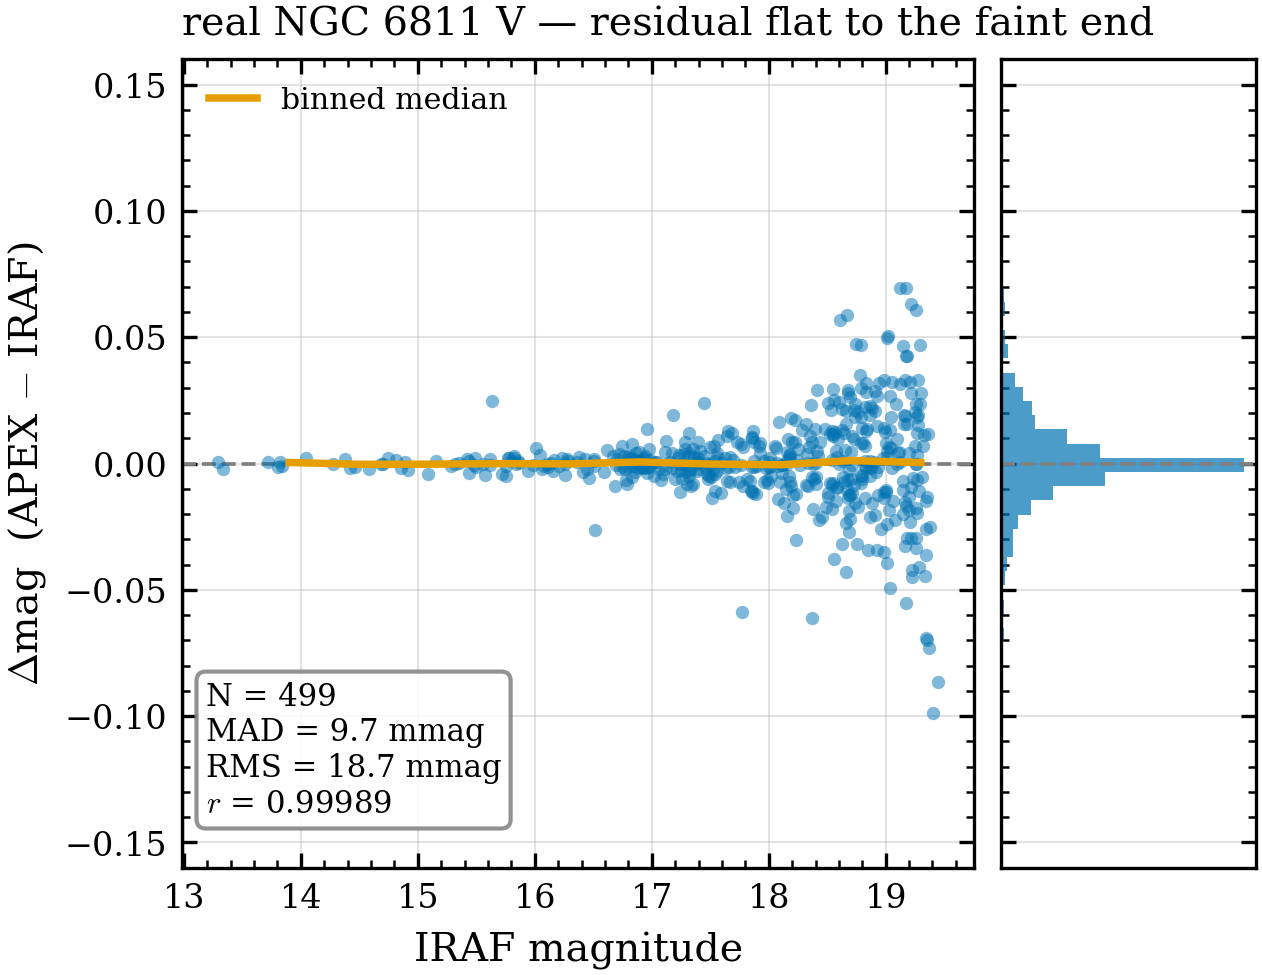
\includegraphics[width=\columnwidth]{fig_iraf_crosscheck.png}
  \caption{APEX versus IRAF/DAOPHOT on 499 real stars in NGC~6811 ($V$ band), a frame reduced from raw entirely by APEX. Both engines measure the same fixed sky coordinates with the matched parameters of Table~\ref{tab:irafparams}. MAD $9.7$ mmag, $r=0.99989$, with the binned median flat to the faint end.}
  \label{fig:irafcheck}
\end{figure}

\begin{table}
  \caption{Parameter matching for the IRAF cross-check. APEX's own values, taken from the frame it had already reduced, were transcribed into the corresponding IRAF tasks so that the residual isolates the two flux integrators rather than a configuration difference. Values are for the NGC~6811 $V$ frame; FWHM-derived quantities follow APEX's scale factors ($0.8$, $4$, $2\times$FWHM).}
  \label{tab:irafparams}
  \begin{tabular}{lll}
    \hline
    Quantity & APEX & IRAF task.parameter \\
    \hline
    PSF FWHM        & 6.146 px            & \texttt{datapars.fwhmpsf} 6.146 \\
    Aperture radius & 4.917 px            & \texttt{photpars.apertures} 4.917 \\
    Sky annulus     & 24.585 px           & \texttt{fitskypars.annulus} 24.585 \\
    Annulus width   & 12.292 px           & \texttt{fitskypars.dannulus} 12.292 \\
    Sky estimator   & clipped median      & \texttt{salgorithm} median, $3\sigma$ \\
    Gain            & 0.681 e$^-$/ADU     & \texttt{datapars.epadu} 0.681 \\
    Read noise      & 2.35 e$^-$          & \texttt{datapars.readnoise} 2.35 \\
    Background $\sigma$ & 30.334 ADU      & \texttt{datapars.sigma} 30.334 \\
    Exposure        & 30 s                & \texttt{datapars.itime} 30 \\
    Zeropoint       & 25.0                & \texttt{photpars.zmag} 25.0 \\
    Recentring      & disabled            & \texttt{calgorithm} none, shift 0 \\
    Noise model     & CCD equation        & \texttt{datapars.noise} poisson \\
    Aperture corr.  & 1.429 applied       & not applied (see text) \\
    \hline
  \end{tabular}
\end{table}

The strongest single accuracy test in this suite measures 499 real stars in NGC~6811 ($V$ band) independently with APEX's forced photometry and with IRAF's \texttt{phot} (DAOPHOT, via PyRAF) at identical fixed sky coordinates (Fig.~\ref{fig:irafcheck}). A comparison between two photometry codes only isolates the codes if everything else is held equal, so APEX's own configuration for that frame --- aperture and annulus radii, gain, read noise, background $\sigma$, exposure time, zeropoint, and the decision not to recentre --- was transcribed into the corresponding IRAF tasks before the run; Table~\ref{tab:irafparams} lists the correspondence. Recentring is disabled on both sides (\texttt{calgorithm}~=~none, maximum shift 0), so both engines integrate flux at the same pixel positions and the residual cannot absorb a centroiding difference. The one deliberate asymmetry is the aperture correction, which APEX applies ($1.429$ for this frame) and IRAF does not; being a single multiplicative constant it appears purely as a zeropoint offset ($-0.049$ mag) and is removed by the same zeropoint alignment used for any inter-code comparison.

After that alignment the two engines agree to MAD $9.7$ mmag, RMS $18.7$ mmag, and Pearson $r=0.99989$, with the binned median residual flat from the bright end to the faint end --- the systematic-attribution check of \citet{schechter1993}. The agreement is best read against the errors the two codes report for themselves: median formal uncertainties of $20.3$ mmag (APEX) and $19.0$ mmag (IRAF) combine in quadrature to $27.8$ mmag, so the measured disagreement between two independently implemented integrators is roughly a third of the scatter their own error models predict. Because this is real observed data on a frame APEX reduced from raw, and because IRAF shares no code with APEX, this tests on-sky correctness rather than internal self-consistency. The same procedure applied to a second cluster and band (NGC~457, $g$, 278 stars) gives MAD $4.3$ mmag; extending the cross-check further across frames and bands remains the most valuable strengthening of the accuracy claim.

\subsection{Frame quality control}
\label{sec:qc}

\begin{figure}
  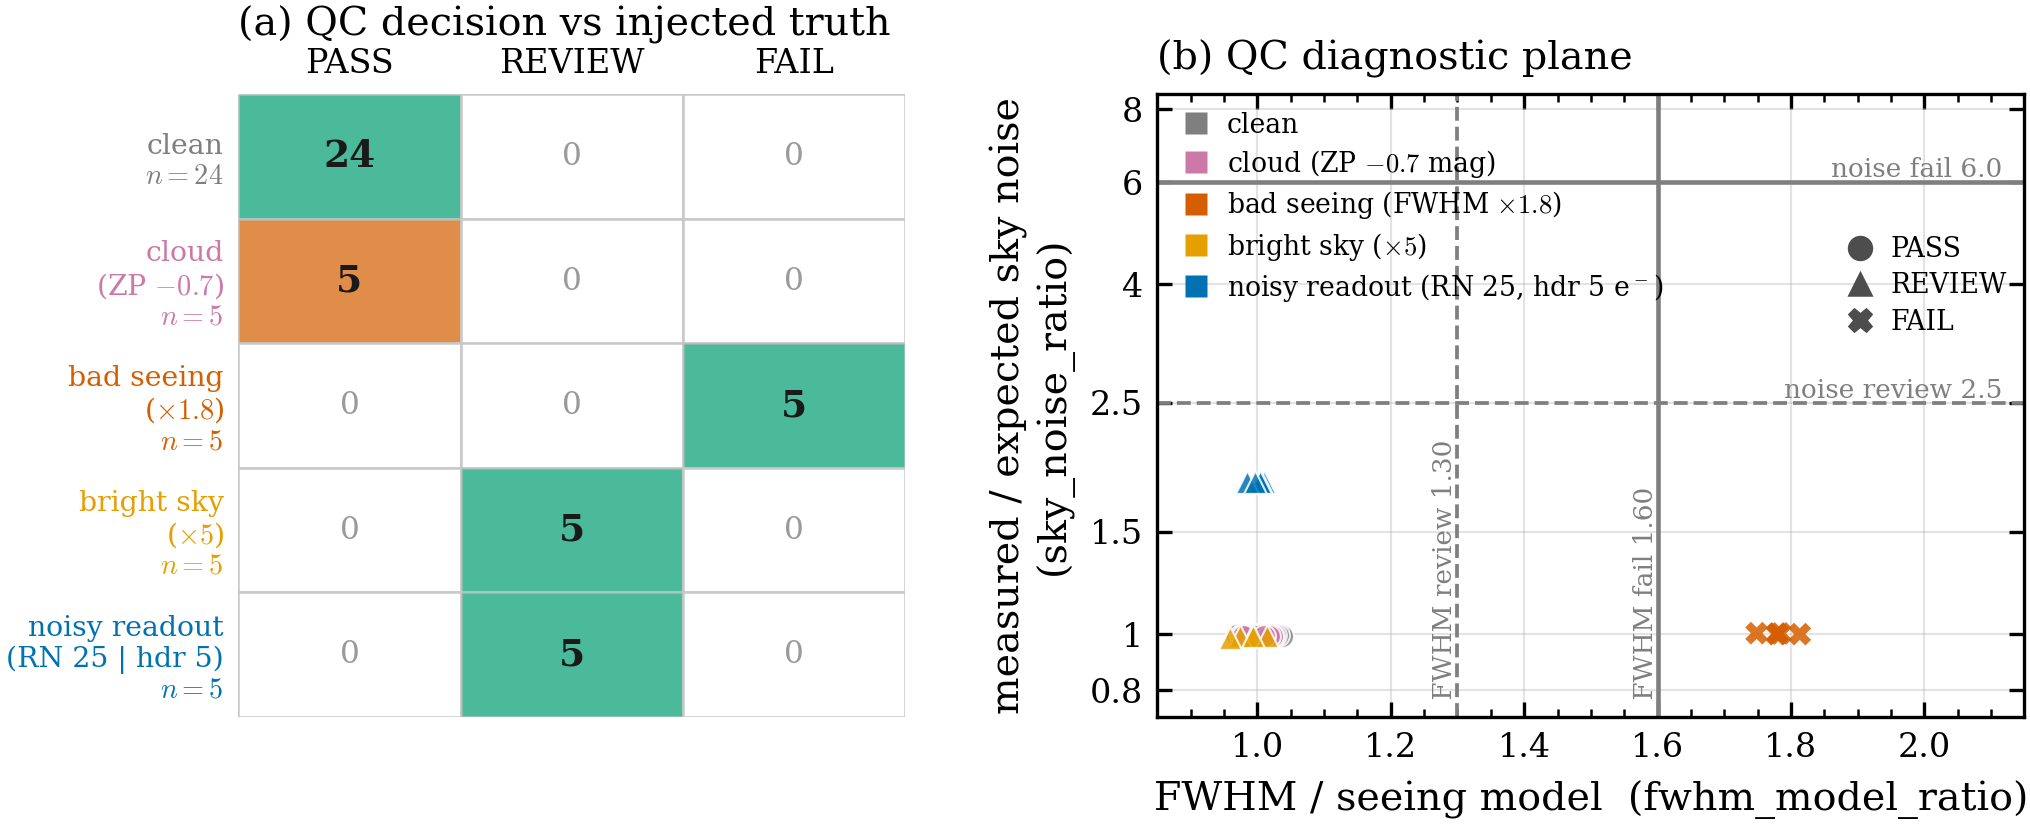
\includegraphics[width=\columnwidth]{fig6_qc_validation.png}
  \caption{Frame-QC on a synthetic 44-frame night. Clean frames pass with no false positives; bad seeing, bright sky, and header-lying noisy readout are caught; grey transparency loss (``cloud'') is a measured structural blind spot.}
  \label{fig:qc}
\end{figure}

Run on a synthetic 44-frame night (24 clean frames plus four defect classes of five frames each), the automatic frame-QC module with its shipped default thresholds passes all 24 clean frames with no false positives, fails all five bad-seeing frames, and flags all five bright-sky and all five header-lying noisy-readout frames for review (Fig.~\ref{fig:qc}). The one class it does not catch is grey transparency loss: all five ``cloud'' frames pass, because a uniform transparency change alters no image-level shape, sky-level, or sky-noise statistic. This is a structural blind spot rather than a defect, and it is the direct motivation for APEX's second-stage, photometry-level transparency check (matched-star frame-offset monitoring), which is positioned to catch exactly this case.

\subsection{Predicted detection depth as a per-frame gate}
\label{sec:depthqc}

\begin{figure*}
  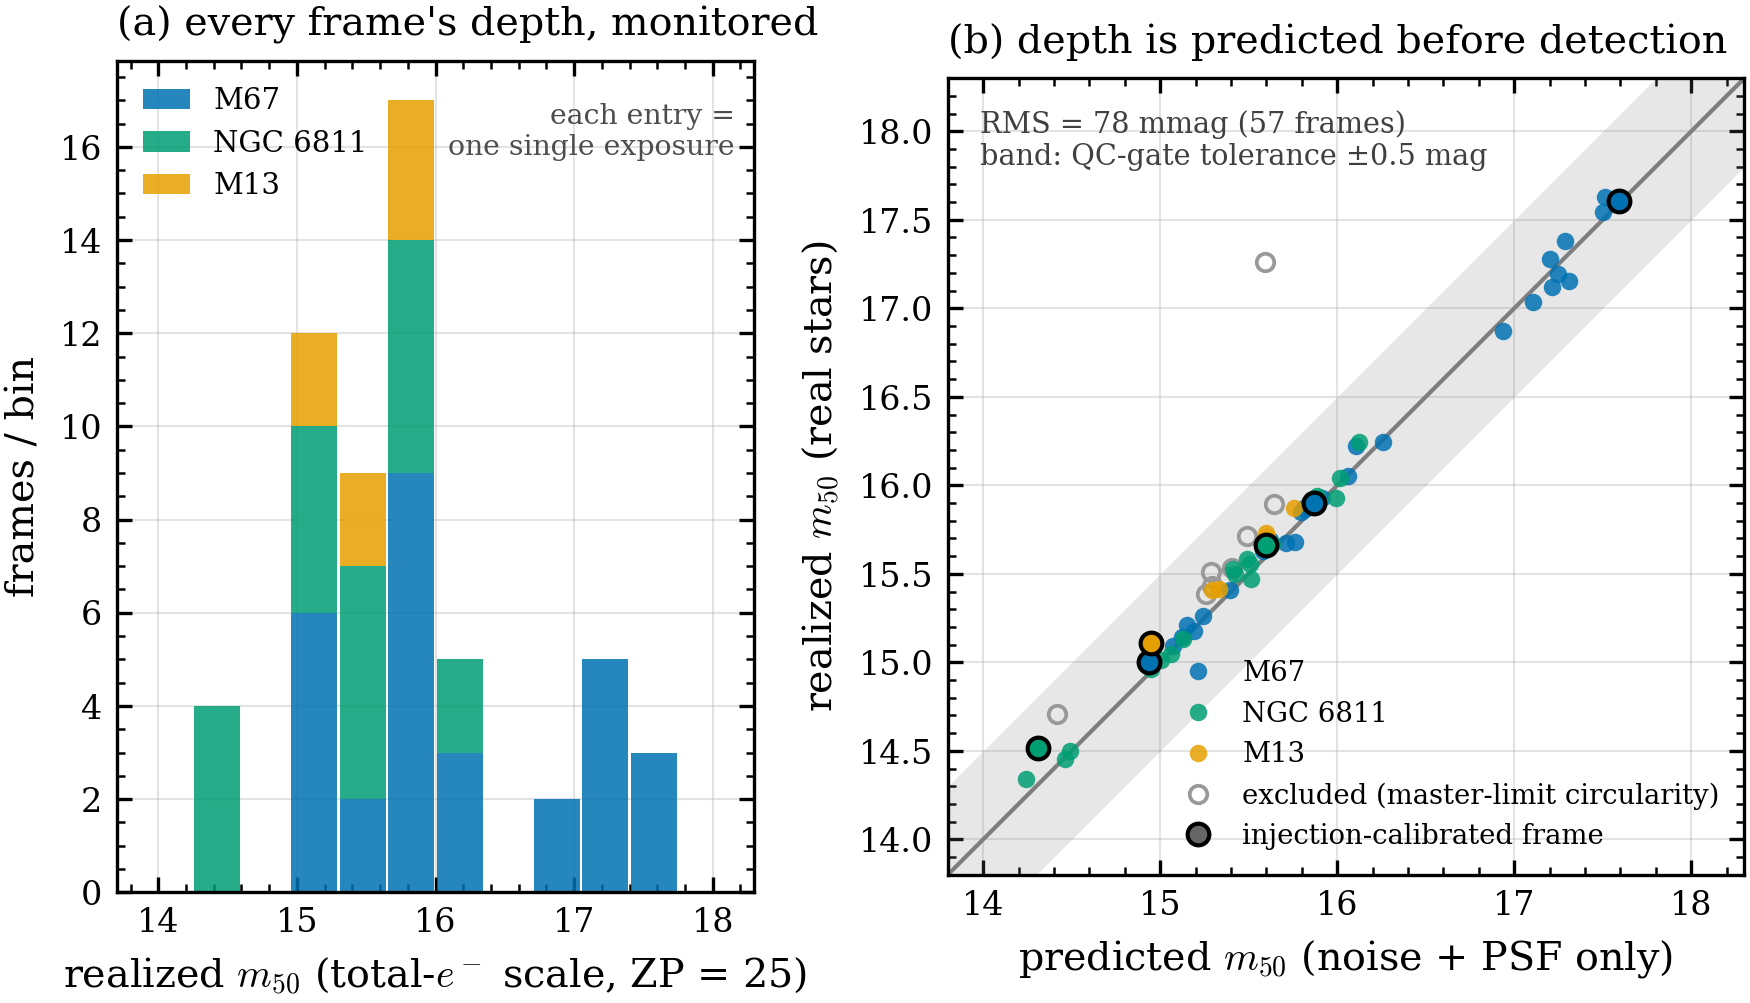
\includegraphics[width=\textwidth]{fig_qc_depth.png}
  \caption{Per-frame detection depth as an operational product, following the fake/known-source monitoring of DES-SN \citep{kessler2015} and ATLAS \citep{tonry2018}. \emph{(a)} Distribution of realized 50 per cent depths over 57 single exposures of three clusters, each entry one frame. \emph{(b)} Depth predicted from a frame's background noise and PSF alone, through the injection-calibrated $\mathrm{S/N}_{50}$ law and before any detection is examined, against the realized depth from real master-catalogue stars: RMS $78$~mmag, all within the $\pm0.5$~mag gate tolerance (shaded). Injection-calibrated frames are ringed; nine frames excluded by a master-catalogue circularity guard are shown open.}
  \label{fig:depthqc}
\end{figure*}

The signal-to-noise law of Section~\ref{sec:completeness} turns detection depth into something APEX can predict for a frame before measuring it, which the pipeline exposes as a per-frame quality gate. From a frame's background noise $\sigma$ and empirical PSF peak fraction $p_{\rm peak}$ alone --- no injection, no image re-read --- the predicted depth is $m_{50}=\mathrm{ZP}-2.5\log_{10}(\mathrm{S/N}_{50}\,\sigma/p_{\rm peak})$ with $\mathrm{S/N}_{50}=4.05$ fixed by the injection experiment above. Across 57 real exposures of three clusters this prediction matches the depth realized from the frame's own recovered master-catalogue stars to an RMS of $78$~mmag, every frame inside the $\pm0.5$~mag gate tolerance (Fig.~\ref{fig:depthqc}); the seven injection-calibrated frames sit on the same relation as the rest, and nine frames whose realized depth approaches the master catalogue's own limit are flagged and excluded by a circularity guard rather than trusted. Presentation-wise this follows the per-epoch depth monitoring that transient surveys run on injected or known sources \citep{kessler2015, tonry2018, anbajagane2025}; the predictive half --- a depth computed from noise and PSF before detection --- is what the gate adds, letting a frame whose detections fall short of its expected depth be flagged for focus, cloud, or defect at ingest.

\subsection{Detection threshold: contamination measured from the frame itself}
\label{sec:threshold}

\begin{figure*}
  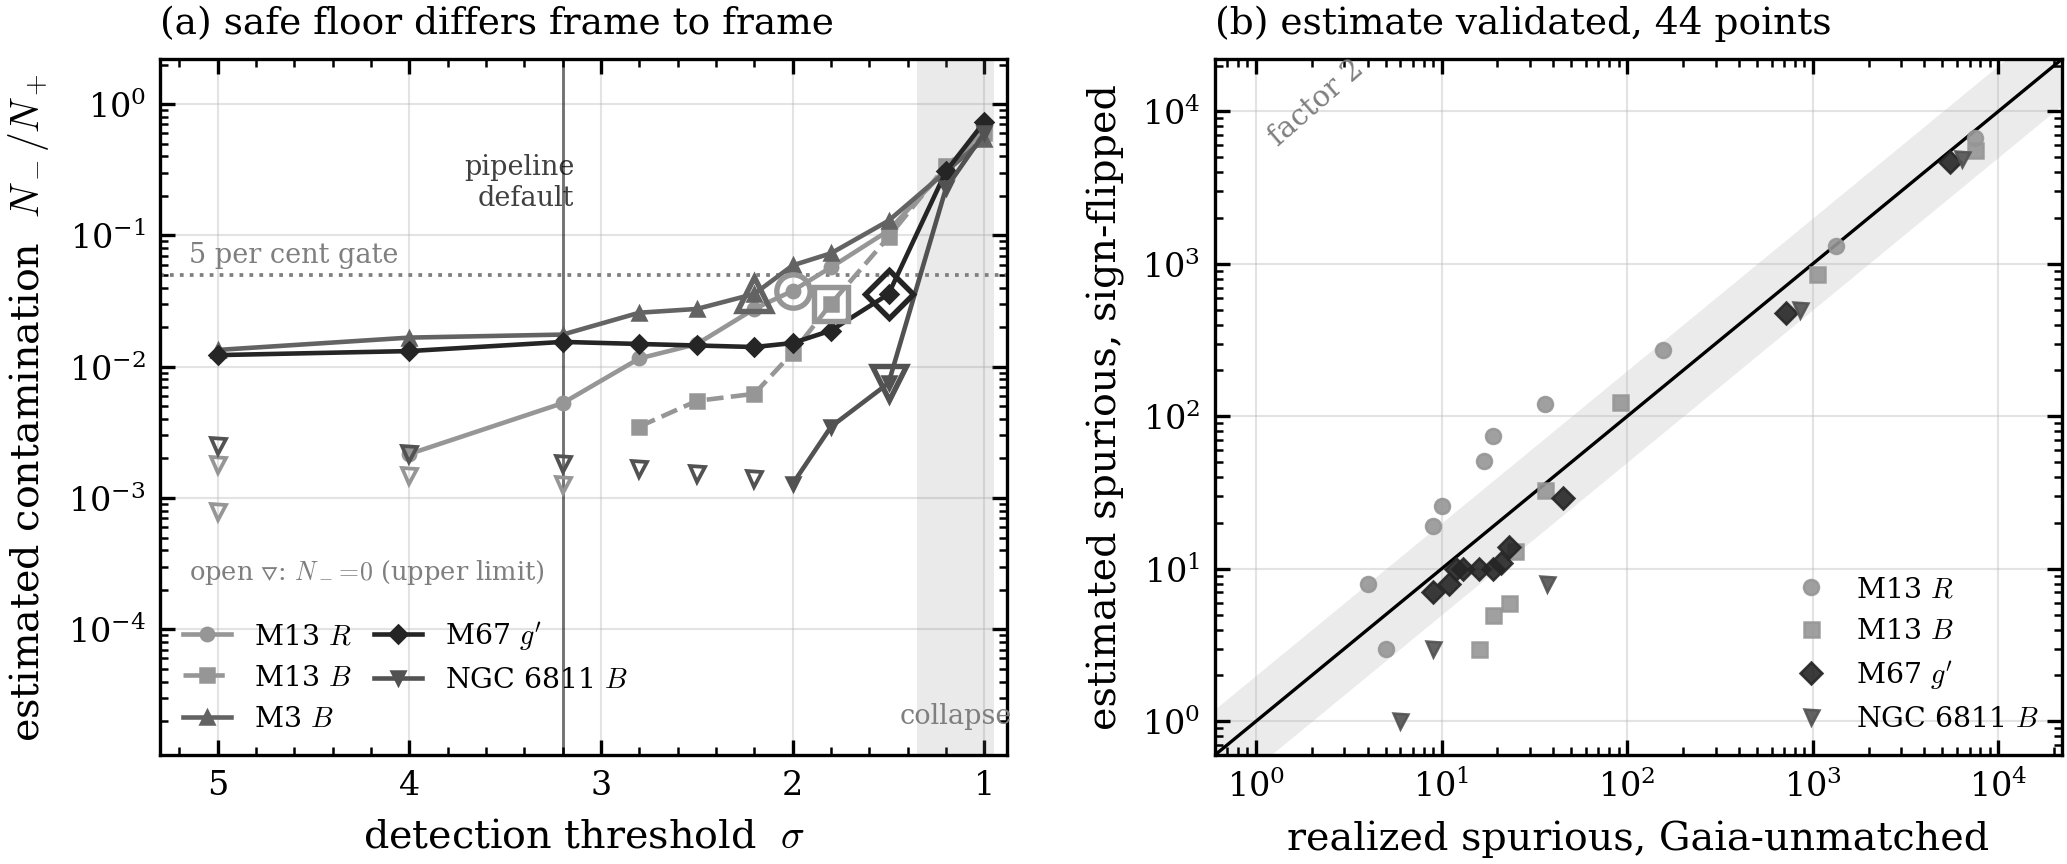
\includegraphics[width=\textwidth]{fig_detection_threshold.png}
  \caption{Spurious contamination against detection threshold, measured without an external catalogue by re-running the detector on the sign-flipped frame \citep{serra2012, molino2014}. \emph{(a)} Five real exposures of four clusters in $B$, $R$ and $g'$. Open carets are upper limits (no detection in the flipped image, plotted at $1/N_+$ and kept out of the line); large open symbols mark each frame's own floor, the lowest threshold holding contamination under 5 per cent. The floors are $1.5,\,1.5,\,1.8,\,2.0,\,2.2$ --- and the two M13 curves split between filters of the same cluster on the same night. All five collapse together between $1.5\sigma$ and $1.2\sigma$ (shaded). \emph{(b)} Validation against Gaia DR3: catalogue-free estimate against the count realized from Gaia non-matches, 44 points over four decades, agreeing to $2.4$ per cent in the collapse region and biased conservative above it.}
  \label{fig:threshold}
\end{figure*}

The detection threshold is the one free parameter upstream of everything else in the measurement chain, and a catalogue built at too low a threshold does not announce itself: the shape and isolation filters of Section~\ref{sec:chain} remove most noise peaks, so the surviving source count looks ordinary. The sweep of Section~\ref{sec:sweep} found the detector threshold-robust, with depth constant to $<0.01$ mag and no spurious detections between $2$ and $6\sigma$, but that was measured on a controlled synthetic field whose uniform background and absence of bright-star wing residuals make threshold robustness look better than it is on sky. We therefore measure the contamination directly, using the property that a background-subtracted frame's noise is symmetric about zero while real sources are positive: re-running the same detector on the sign-flipped image counts the noise-origin spurious detections, and $(N_+-N_-)/N_+$ estimates the purity. The technique is standard in radio and sub-millimetre source finding, where it assigns a per-source reliability from the density of negative detections in parameter space \citep{serra2012, serra2015}, and has been used on optical images to choose a threshold at fixed contamination \citep{molino2014}; the alternative of setting the threshold by controlling the false-discovery rate \citep{hopkins2002} operates per pixel and does not compose with the minimum-connected-area criterion used here. Because it needs neither a WCS solution nor an injection, the measurement runs inside the detection step, before plate solving, for 0.21~s on a $4788\times3194$ frame --- 3.6 per cent of that step.

The symmetry the method rests on holds for these frames but was checked rather than assumed, since an optical image is everywhere positive before background subtraction. After subtraction the pixel distribution has skewness $+0.058$ (M13~$R$) and $+0.051$ (NGC~6811~$B$) against the Poisson expectations $+0.045$ and $+0.048$ at those sky levels ($\sim$500~$e^-$\,px$^{-1}$), with a median offset of $0.02\sigma$. At the shipped $3.2\sigma$ default all five frames of Fig.~\ref{fig:threshold}a sit at or below 2 per cent contamination, and the estimate is validated against Gaia DR3 to within a factor of two over four decades, agreeing to 2.4 per cent where the counts are largest (Fig.~\ref{fig:threshold}b). Lowering the threshold is safe for some distance --- every frame here remains under 5 per cent to at least $2.2\sigma$ --- and then all five collapse together between $1.5\sigma$ and $1.2\sigma$, at $1.2\sigma$ yielding 4066 detections of which 1341 are spurious. That the collapse is common while the safe floor is not follows from what each depends on: the probability that noise clears the threshold over the minimum connected area is a property of the threshold alone, whereas the floor also depends on how many real sources the frame contributes to $N_+$.

Two consequences are worth separating. The first is that a single threshold chosen once for a programme is not equivalent to a threshold chosen per frame: the floors here span $1.5$--$2.2\sigma$, and the split between M13~$R$ and M13~$B$ shows this happening within one cluster on one night, so it cannot be assigned to the target. The second is a limit of the test rather than of the pipeline. Cosmic rays, hot pixels and satellite trails are positive-only and have no negative counterpart, so this measurement is blind to them by construction; they are the province of the separate rejection stage, and the quantity reported here is specifically \emph{noise-origin} contamination. Operationally APEX records the threshold actually used with each frame's detection products alongside the raw extractor yield, so a catalogue built at a lowered threshold remains identifiable after the fact; the measurement above is what supplies the missing half, a scale on which a given yield can be judged. Finally, these five frames come from one camera, and the floors quoted are not a recommendation transferable to another instrument.

\subsection{Reference-catalogue cross-validation: a reference artifact, not an APEX error}
\label{sec:refcheck}

\begin{figure}
  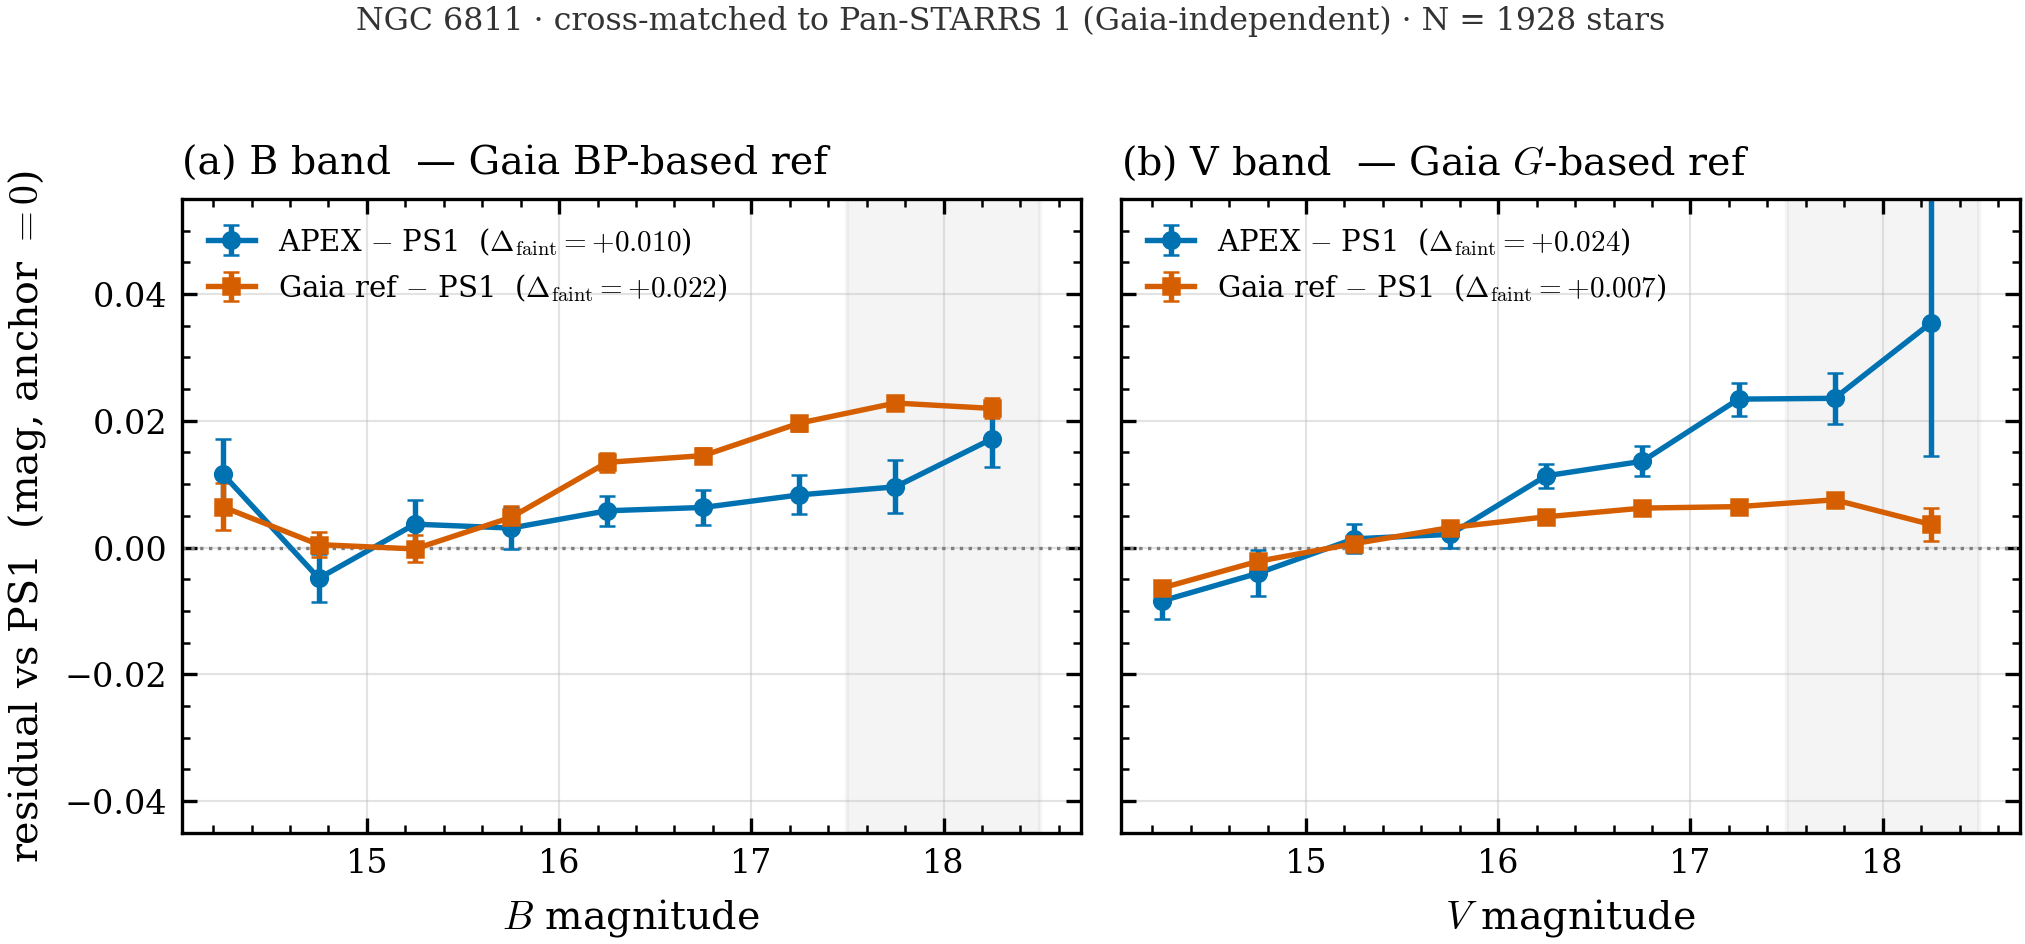
\includegraphics[width=\columnwidth]{fig7_reference_crosscheck.png}
  \caption{NGC~6811 against Pan-STARRS~1, independent of Gaia. The dominant faint-end systematic swaps catalogue between $B$ and $V$, isolating a Gaia BP reference artifact from APEX's own residual.}
  \label{fig:refcheck}
\end{figure}

Cross-matching 1928 NGC~6811 stars to Pan-STARRS~1 \citep{chambers2016}, fully independent of Gaia, separates a \emph{reference} systematic from a \emph{measurement} systematic band by band (Fig.~\ref{fig:refcheck}). In $B$, the Gaia-transformed reference drifts $+0.022$ mag against PS1 toward faint magnitudes, larger than APEX's own $+0.010$ mag; in $V$ the pattern reverses, with the Gaia reference flat ($+0.007$) and APEX carrying a small $+0.024$ mag residual. The dominant systematic swaps catalogue between bands, which is only possible if the two are independent. In $B$ the culprit is Gaia's BP channel, whose flux is background-dominated and biased for faint blue sources \citep{riello2021}; APEX's own $B$, checked against the independent PS1 scale, is flat to $\sim0.01$ mag. The faint ``$B$-band drift'' first seen against Gaia is therefore chiefly a reference artifact. The practical lesson is that bright-star Gaia anchoring remains safe for the zeropoint, but faint-end \emph{validation} should use a $G$-based or PS1 reference rather than BP-transformed magnitudes.

\subsection{CMD reproduction across independent photometric systems}
\label{sec:cmd}

\begin{figure}
  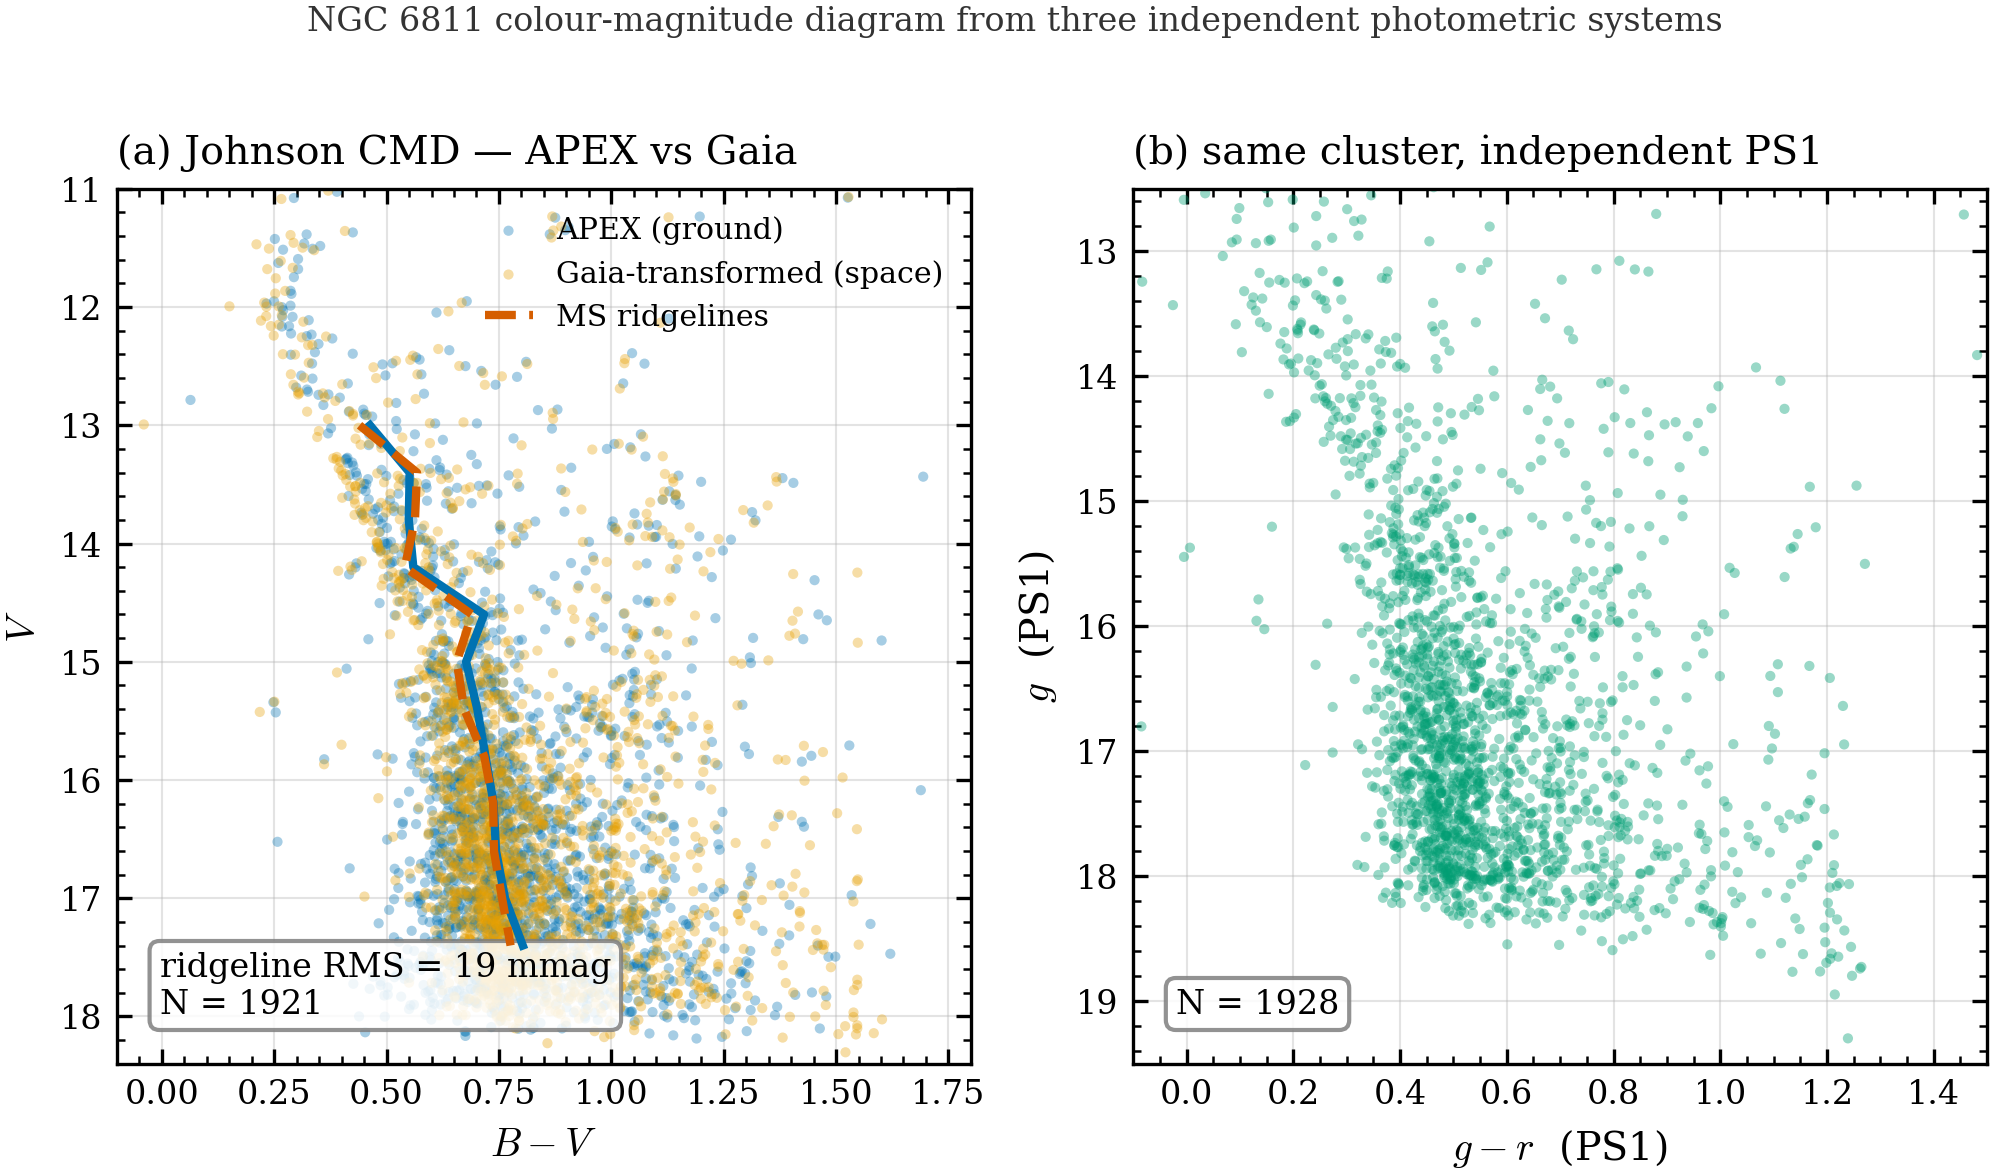
\includegraphics[width=\columnwidth]{fig8_cmd_reproduction.png}
  \caption{The NGC~6811 CMD from APEX ground-based photometry overlaid on a Gaia-transformed reference (ridgelines agree to 19 mmag), and the same cluster in the independent PS1 system.}
  \label{fig:cmd}
\end{figure}

The colour--magnitude diagram, the CMD-mode science product, is validated without fitting anything (Fig.~\ref{fig:cmd}). The NGC~6811 Johnson CMD ($V$ vs $B-V$, 1921 stars) from APEX ground-based aperture photometry overlays the Gaia-transformed, space-based reference with sigma-clipped main-sequence ridgelines coinciding to 19 mmag RMS; the same cluster in the independent PS1 system shows the identical morphology. This validates the CMD \emph{product}, not isochrone \emph{fitting}: recovering age, metallicity, distance, and reddening from a single-colour ground-based CMD is a known-degenerate inverse problem (Section~\ref{sec:outofscope}), which we treat separately and do not claim here.

\subsection{Crowded-field replication in two globular clusters}
\label{sec:crowding}

\begin{figure}
  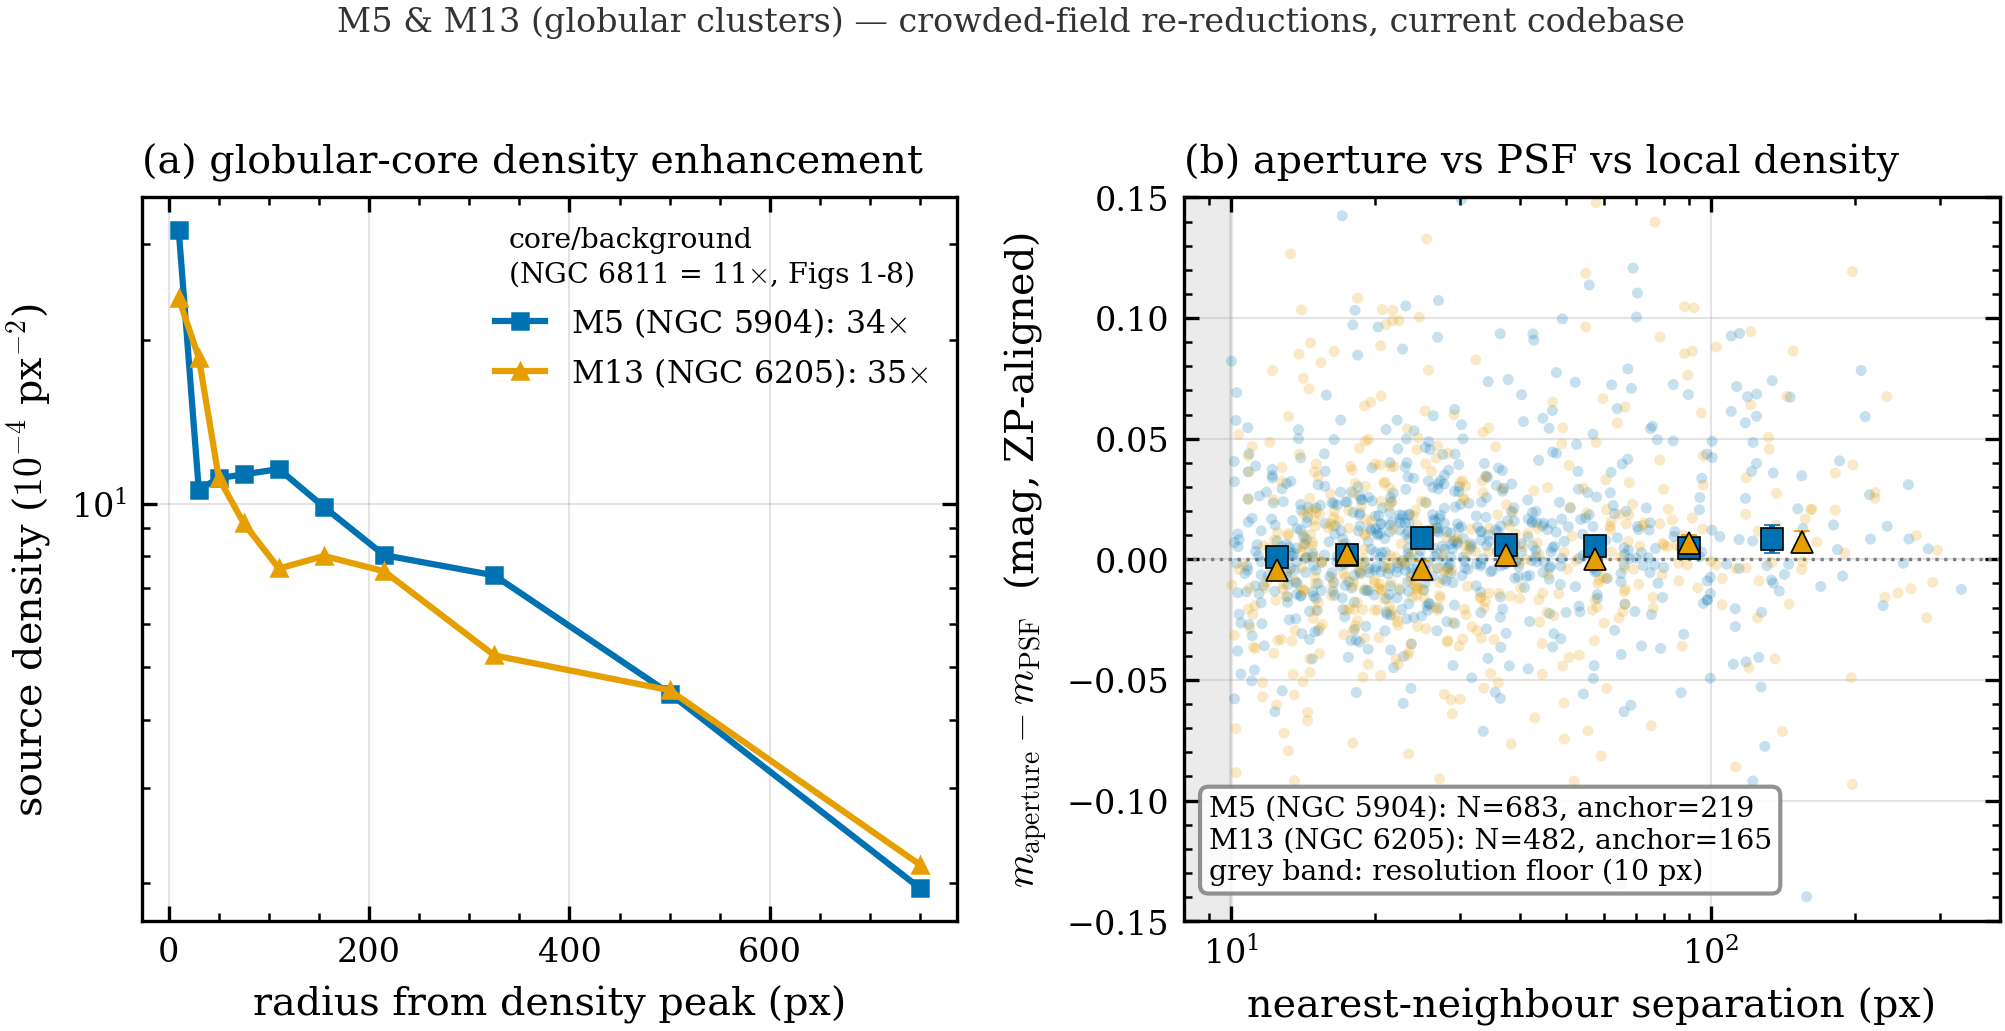
\includegraphics[width=\columnwidth]{fig9_crowded_field.png}
  \caption{Aperture-versus-PSF residual against nearest-neighbour separation in M5 and M13 (core densities $34\times$ and $35\times$ background). The binned medians are flat in both, from the resolution floor ($\sim$10 px, $\sim$4$''$) outward.}
  \label{fig:crowding}
\end{figure}

The synthetic experiments use uncrowded fields; this test extends into two real globular-cluster cores and asks whether the result replicates (Fig.~\ref{fig:crowding}). Using APEX's own density-peak finder, M5's core is enhanced $34\times$ and M13's $35\times$ over their field backgrounds, both far above NGC~6811's $11\times$ by the same metric. The probe shown is deliberately Gaia-independent: it compares APEX's own two measurement methods, forced aperture versus PSF photometry, on the same matched star list as a function of nearest-neighbour separation. This is an \emph{internal-consistency} test --- it bounds how much crowding can make the two methods disagree, not an external accuracy check --- and that framing is what makes it robust here, because M13's archived Gaia cross-match is essentially broken (only 38 of 1347 sources resolve in a live Gaia DR3 query) yet the internal comparison needs no Gaia identity. The binned aperture-minus-PSF medians are flat in both clusters, consistent with zero within $\pm0.02$--$0.04$ mag from the resolution floor ($\sim$10 px, $\sim$4$''$) out to isolated separations. Within the separation this ground-based, $2\times2$-binned instrument resolves, no crowding-dependent disagreement between the two methods is detected, and the null result replicates across two independently reduced fields. Sub-resolution blending finer than this dataset resolves is not and cannot be tested here, and remains open.

% ============================================================================
\section{Science application: a variable-star light curve}
\label{sec:science}

\begin{figure*}
  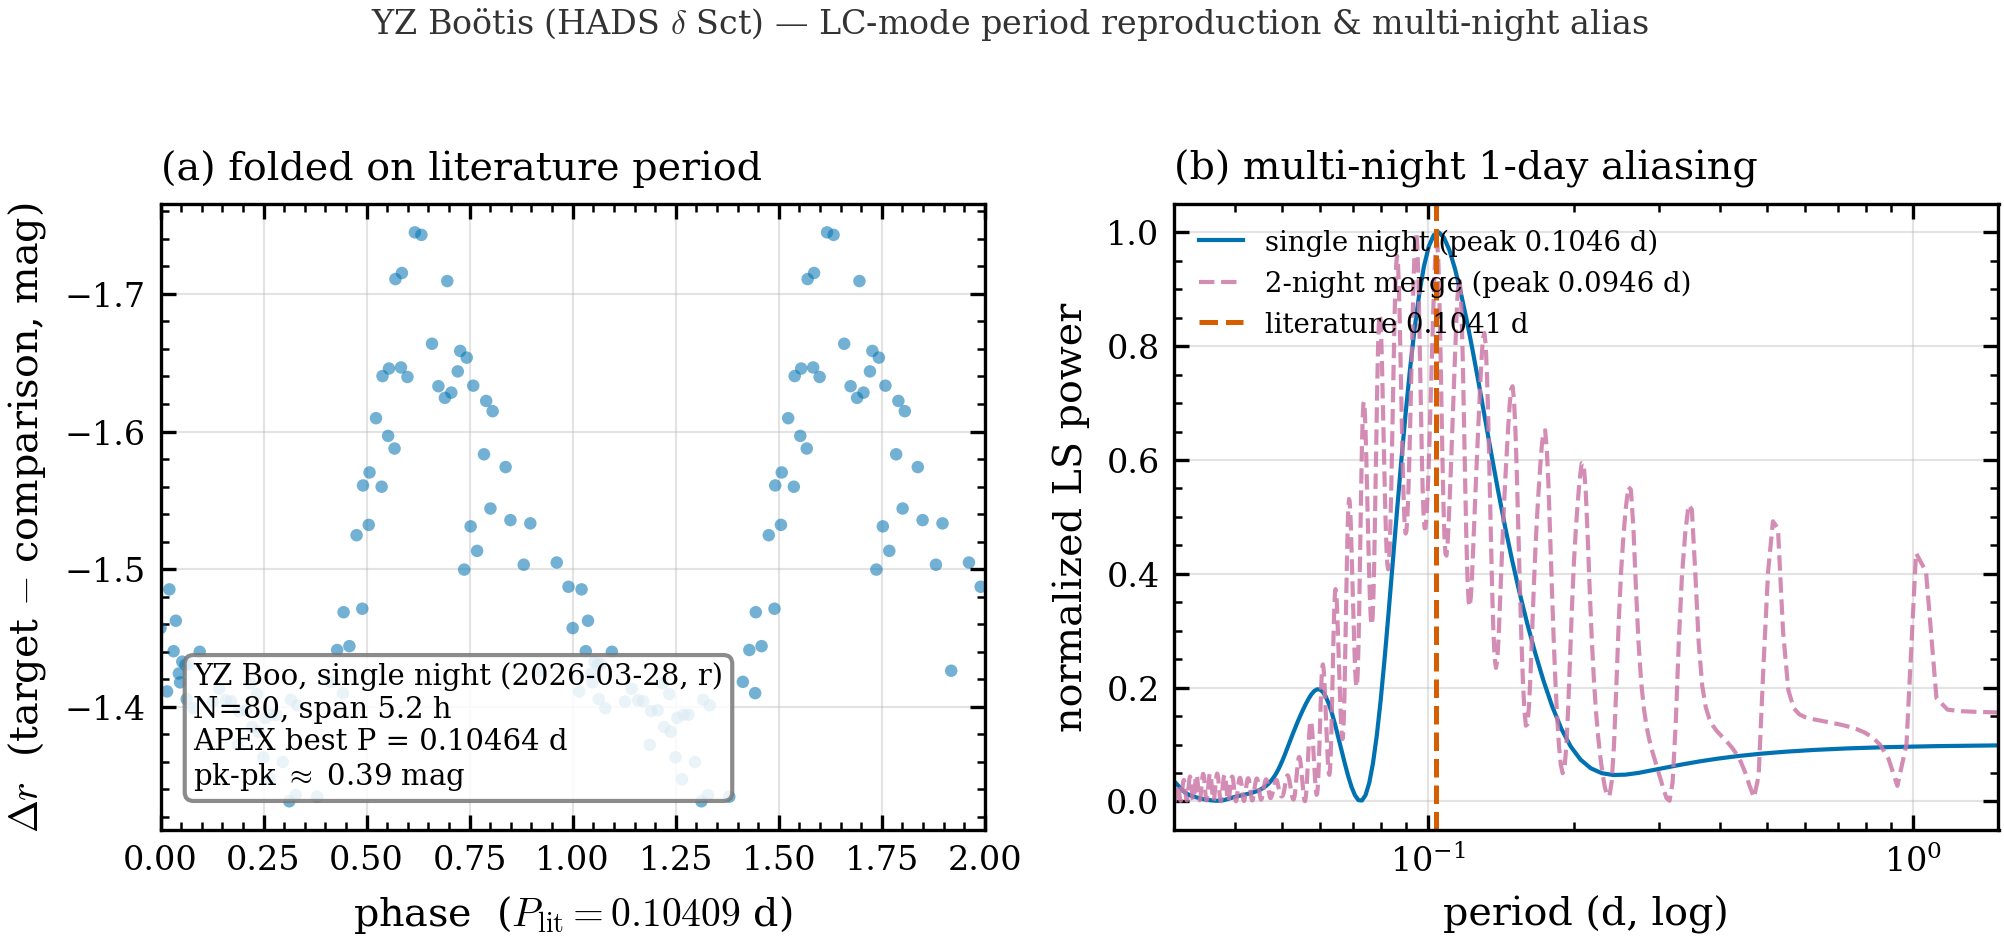
\includegraphics[width=\textwidth]{fig_lc_yzboo.png}
  \caption{End-to-end science product from LC mode: the high-amplitude $\delta$~Scuti star YZ~Bo\"otis, reduced from raw frames entirely within APEX. \emph{(a)} One night (2026-03-28, $r$ band, $N=80$ over 5.2~h) folded on the literature period, reproducing the published sawtooth with a peak-to-peak amplitude of $0.39$ mag. \emph{(b)} Lomb--Scargle periodograms: the single night peaks at $0.1046$~d, within 0.5 per cent of the literature $0.10409$~d (dashed), while merging two nights separated by a one-day gap moves the highest peak to $0.0946$~d --- the $+1$~c/d alias --- leaving the true period as a secondary peak. The alias is a property of the observing window, not of the pipeline, and is shown rather than hidden.}
  \label{fig:lcyzboo}
\end{figure*}

The validation above establishes that the measurement chain is accurate; this section asks the question a user actually has, which is whether that accuracy survives all the way to a published quantity. We reduced the high-amplitude $\delta$~Scuti star YZ~Bo\"otis (literature period $P = 0.104092$ d, $V$ peak-to-peak $\simeq 0.42$ mag; \citealt{yang2018}) from raw frames to a period, entirely inside APEX's LC mode and through the graphical workflow, with no scripting at any step.

A single night --- 2026-03-28, $r$ band, 80 differential measurements spanning 5.2~h --- folds on the literature period into the published sawtooth (Fig.~\ref{fig:lcyzboo}a) with a peak-to-peak amplitude of $0.392$ mag. The amplitude being smaller than the catalogued $V$ value is expected rather than discrepant: pulsation amplitude in $\delta$~Scuti stars decreases toward longer wavelengths, so an $r$-band amplitude below the $V$-band one is the physically correct ordering. Run blind, without assuming the answer, a Lomb--Scargle periodogram \citep{vanderplas2018} of that night peaks at $P = 0.10464$~d, which is $0.5$ per cent (47~s) from the literature value. The night spans only 2.1 pulsation cycles, so this is a short-baseline estimate and we do not present it as a refinement of the published ephemeris; the point is that a non-scripting user, starting from raw frames, arrives at the right star with the right period and the right amplitude.

The second panel is the honest half. Merging that night with another separated by a one-day gap moves the highest periodogram peak to $0.0946$~d, the $+1$~cycle/day alias, with the true period surviving only as a secondary peak. This is the standard spectral-window aliasing of single-site ground-based photometry, and it is a property of when the data were taken rather than of how they were reduced --- no pipeline removes it. We report it because it defines where the user's judgement is still required: APEX presents the periodogram and the folded curve, it does not adjudicate between aliases. That division is deliberate and is the same one the frame-quality gate makes (Section~\ref{sec:depthqc}), where the pipeline flags a frame whose depth falls short of prediction but leaves the decision with the observer.

The dual-mode pulsator AE~Ursae Majoris \citep{zhou2001, paparo2001} is noted as future work: separating its fundamental and first-overtone modes requires prewhitening not yet implemented in APEX, and with single-site aliasing the highest peak is an unreliable estimate of the true fundamental for such a star.

% ============================================================================
\section{Discussion}
\label{sec:discussion}

\subsection{What is established}

Across Sections~\ref{sec:completeness}--\ref{sec:cmd}, APEX's aperture and PSF measurement, from detection through forced photometry and automatic frame quality control, behaves as a well-calibrated instrument. Its detection depth is set by each frame's sky and seeing through a single signal-to-noise threshold, one the pipeline predicts per frame from noise and PSF alone to $78$~mmag and exposes as a quality gate (Sections~\ref{sec:completeness}, \ref{sec:depthqc}). Reported uncertainties propagate correctly (Section~\ref{sec:errormodel}); two independently implemented engines and an independent real-data reference agree at the milli-magnitude level (Sections~\ref{sec:sepcheck}--\ref{sec:irafcheck}); pipeline and observing-condition parameters move the metrics in the physically expected directions (Section~\ref{sec:sweep}); and the resulting colour--magnitude diagram is indistinguishable from what two other instruments produce for the same stars (Section~\ref{sec:cmd}). The one apparent measurement anomaly investigated in depth, a faint-end $B$-band drift, resolved to a documented weakness of the external reference rather than of APEX (Section~\ref{sec:refcheck}). Extended into two crowded real fields, the pipeline continues to perform correctly and the null crowding result replicates (Section~\ref{sec:crowding}), with the honest qualifier that this is an internal aperture-versus-PSF consistency bound down to the resolution this dataset reaches, not a proof that aperture photometry is crowding-proof at arbitrary separations.

\subsection{What is out of scope by construction}
\label{sec:outofscope}

Automated isochrone-parameter recovery (age, metallicity, distance, reddening) is not validated here. It is a known-degenerate inverse problem for ground-based single- or dual-colour photometry: unconstrained fits rail toward spuriously metal-poor, short-distance solutions, and even with external priors the metallicity retains a bias absent a spectroscopic or blue-band constraint. This is a property of the astrophysical degeneracy and the fit likelihood (cf.\ the $\tau^2$ CMD-fitting framework of \citealt{naylor2006}), not a photometric-accuracy statement about the measurements validated here; Section~\ref{sec:cmd} accordingly validates the CMD product, not its interpretation. The light-curve mode is exercised end to end in Section~\ref{sec:science}, and is validated only to the extent that section establishes.

\subsection{Limits on generality}
\label{sec:generality}

\paragraph*{Single instrument (verified, not assumed).} Every real dataset used in Sections~\ref{sec:irafcheck} and~\ref{sec:refcheck}--\ref{sec:crowding} was taken with the identical camera; the genuine independence axes in this paper are the cross-check \emph{methods} (SEP, IRAF/DAOPHOT, Gaia, Pan-STARRS~1), which carry no APEX-camera-specific assumption, not the choice of cluster. A second telescope and camera reduced with APEX remains the strongest open generality test.

\paragraph*{Structured sky background.} APEX estimates the sky in a sigma-clipped annulus, which assumes the background is locally uniform on the scale of the aperture and annulus. This holds for stars on blank sky and is adequate for the smooth, slowly varying backgrounds of the cluster fields used here, where a gentle gradient is largely absorbed by the annulus median. It fails where the background carries structure on the scale of the aperture itself: bright nebular emission, Galactic cirrus, or a star superimposed on resolved galaxy light. There the annulus mis-estimates the true background beneath the source and the photometry is biased in a position-dependent way. This regime is neither used nor validated here, and it is distinct from the stellar crowding of Section~\ref{sec:crowding}, which is source confusion rather than diffuse background. Photometry of variables or transients embedded in host-galaxy or strong nebular emission would require spatially resolved background modelling or template subtraction, as AutoPhOT performs for transients in galaxies \citep{brennan2022}, which APEX does not currently do. The variable-star target of Section~\ref{sec:science} is a Galactic field pulsator in a comparatively clean field, so this limitation does not affect the results reported here.

\paragraph*{Sub-resolution crowding.} Section~\ref{sec:crowding} finds no crowding-dependent bias down to the $\sim$10 px ($\sim$4$''$) separation this ground-based, $2\times2$-binned dataset resolves. Finer, sub-resolution blending, as would be probed by space-based or lucky imaging, remains untested and is exactly where aperture photometry is still expected to degrade relative to simultaneous PSF fitting.

\paragraph*{A broken external cross-match need not mean broken measurement.} M13's archived, older-pipeline Gaia cross-match is essentially unusable for absolute calibration (only 38 of 1347 detected sources resolve in a live Gaia DR3 query), yet it remained fully usable for the internal, Gaia-independent aperture-versus-PSF test of Section~\ref{sec:crowding}, since forced photometry needs only master-catalogue pixel positions, not a Gaia identity.

\subsection{Practical recommendations}

Use an aperture near $1.0$--$1.2\times$FWHM; the shipped default is already close to the empirical optimum (Section~\ref{sec:sweep}). Treat frame QC as two-stage: the image-level checks validated in Section~\ref{sec:qc} cannot detect grey transparency loss, so a photometry-level (matched-star flux) check is required for that failure mode. For faint-end photometric \emph{validation} specifically (not zeropoint anchoring), prefer a $G$-based or Pan-STARRS reference over BP-transformed Gaia magnitudes (Section~\ref{sec:refcheck}). In crowded fields, prefer an internal aperture-versus-PSF diagnostic over Gaia-matched calibrator statistics, since Gaia's own quality cuts remove the worst blends before they are counted (Section~\ref{sec:crowding}). In fields with strong nebulosity or resolved galaxy light, prefer local background modelling or template subtraction; the annulus sky estimator is intended for stellar fields (Section~\ref{sec:generality}).

% ============================================================================
\section{Conclusion}
\label{sec:conclusion}

By the evidence assembled here, APEX's shared photometric measurement chain is a validated, honestly-erred, cross-checked instrument for aperture and PSF photometry of point sources, from uncrowded open-cluster fields to real globular-cluster cores, and its CMD-mode product reproduces what independent instruments see for the same stars. This is a claim about \emph{measurement}, deliberately scoped away from automated isochrone-parameter recovery, from photometry against strongly structured backgrounds, from sub-resolution blending, and from instruments not yet re-verified against the current code. The contribution of APEX is to make that validated measurement chain reachable, through a graphical workflow, by observers for whom the established command-line tools have been out of reach, and to have shown, rather than asserted, that the accessibility need not cost accuracy within the regime established here.

% ============================================================================
\section*{Data availability}
The APEX source code is available at [REPOSITORY URL] under the MIT licence. The validation suite reproduces every figure via \texttt{run\_all.py}; self-contained figures regenerate from fixed seeds with no external data, while the real-data figures require the observation volume. The Pan-STARRS cross-match is cached with the repository.

\section*{Acknowledgements}
% TODO: acknowledgements, funding, facilities (Moravian C3-61000 camera), software (Astropy, photutils, SEP, IRAF/DAOPHOT, ASTAP, astrometry.net).

\section*{AI-usage disclosure}
% TODO: generate with ars-disclosure for RASTI. Balanced frame: AI-assisted
% development lowered the barrier to building the tool; all scientific claims
% are independently validated (Section 3).

% ============================================================================
\bibliographystyle{mnras}
\bibliography{references}

\bsp
\label{lastpage}
\end{document}
